% Options for packages loaded elsewhere
\PassOptionsToPackage{unicode}{hyperref}
\PassOptionsToPackage{hyphens}{url}
%
\documentclass[
  12pt,
]{article}
\usepackage{amsmath,amssymb}
\usepackage{iftex}
\ifPDFTeX
  \usepackage[T1]{fontenc}
  \usepackage[utf8]{inputenc}
  \usepackage{textcomp} % provide euro and other symbols
\else % if luatex or xetex
  \usepackage{unicode-math} % this also loads fontspec
  \defaultfontfeatures{Scale=MatchLowercase}
  \defaultfontfeatures[\rmfamily]{Ligatures=TeX,Scale=1}
\fi
\usepackage{lmodern}
\ifPDFTeX\else
  % xetex/luatex font selection
\fi
% Use upquote if available, for straight quotes in verbatim environments
\IfFileExists{upquote.sty}{\usepackage{upquote}}{}
\IfFileExists{microtype.sty}{% use microtype if available
  \usepackage[]{microtype}
  \UseMicrotypeSet[protrusion]{basicmath} % disable protrusion for tt fonts
}{}
\makeatletter
\@ifundefined{KOMAClassName}{% if non-KOMA class
  \IfFileExists{parskip.sty}{%
    \usepackage{parskip}
  }{% else
    \setlength{\parindent}{0pt}
    \setlength{\parskip}{6pt plus 2pt minus 1pt}}
}{% if KOMA class
  \KOMAoptions{parskip=half}}
\makeatother
\usepackage{xcolor}
\usepackage[margin=1in]{geometry}
\usepackage{longtable,booktabs,array}
\usepackage{calc} % for calculating minipage widths
% Correct order of tables after \paragraph or \subparagraph
\usepackage{etoolbox}
\makeatletter
\patchcmd\longtable{\par}{\if@noskipsec\mbox{}\fi\par}{}{}
\makeatother
% Allow footnotes in longtable head/foot
\IfFileExists{footnotehyper.sty}{\usepackage{footnotehyper}}{\usepackage{footnote}}
\makesavenoteenv{longtable}
\usepackage{graphicx}
\makeatletter
\def\maxwidth{\ifdim\Gin@nat@width>\linewidth\linewidth\else\Gin@nat@width\fi}
\def\maxheight{\ifdim\Gin@nat@height>\textheight\textheight\else\Gin@nat@height\fi}
\makeatother
% Scale images if necessary, so that they will not overflow the page
% margins by default, and it is still possible to overwrite the defaults
% using explicit options in \includegraphics[width, height, ...]{}
\setkeys{Gin}{width=\maxwidth,height=\maxheight,keepaspectratio}
% Set default figure placement to htbp
\makeatletter
\def\fps@figure{htbp}
\makeatother
\setlength{\emergencystretch}{3em} % prevent overfull lines
\providecommand{\tightlist}{%
  \setlength{\itemsep}{0pt}\setlength{\parskip}{0pt}}
\setcounter{secnumdepth}{5}
% definitions for citeproc citations
\NewDocumentCommand\citeproctext{}{}
\NewDocumentCommand\citeproc{mm}{%
  \begingroup\def\citeproctext{#2}\cite{#1}\endgroup}
\makeatletter
 % allow citations to break across lines
 \let\@cite@ofmt\@firstofone
 % avoid brackets around text for \cite:
 \def\@biblabel#1{}
 \def\@cite#1#2{{#1\if@tempswa , #2\fi}}
\makeatother
\newlength{\cslhangindent}
\setlength{\cslhangindent}{1.5em}
\newlength{\csllabelwidth}
\setlength{\csllabelwidth}{3em}
\newenvironment{CSLReferences}[2] % #1 hanging-indent, #2 entry-spacing
 {\begin{list}{}{%
  \setlength{\itemindent}{0pt}
  \setlength{\leftmargin}{0pt}
  \setlength{\parsep}{0pt}
  % turn on hanging indent if param 1 is 1
  \ifodd #1
   \setlength{\leftmargin}{\cslhangindent}
   \setlength{\itemindent}{-1\cslhangindent}
  \fi
  % set entry spacing
  \setlength{\itemsep}{#2\baselineskip}}}
 {\end{list}}
\usepackage{calc}
\newcommand{\CSLBlock}[1]{\hfill\break\parbox[t]{\linewidth}{\strut\ignorespaces#1\strut}}
\newcommand{\CSLLeftMargin}[1]{\parbox[t]{\csllabelwidth}{\strut#1\strut}}
\newcommand{\CSLRightInline}[1]{\parbox[t]{\linewidth - \csllabelwidth}{\strut#1\strut}}
\newcommand{\CSLIndent}[1]{\hspace{\cslhangindent}#1}
\usepackage{setspace} \usepackage{lineno} \usepackage{placeins} \usepackage[nottoc,notlof,notlot]{tocbibind} \renewcommand{\contentsname}{} \renewcommand{\listfigurename}{} \renewcommand{\listtablename}{} \usepackage{sectsty} \sectionfont{\centering}
\ifLuaTeX
  \usepackage{selnolig}  % disable illegal ligatures
\fi
\usepackage{bookmark}
\IfFileExists{xurl.sty}{\usepackage{xurl}}{} % add URL line breaks if available
\urlstyle{same}
\hypersetup{
  hidelinks,
  pdfcreator={LaTeX via pandoc}}

\author{}
\date{\vspace{-2.5em}}

\begin{document}

\doublespacing

\begin{center}
    
\textbf{\Large Applying effective environmental forecasts to Management Strategy Evaluation of yellowtail flounder}
    
\textsc{Sophie Wulfing$^{1*}$ Chengxue Li$^{3}$ Scott I. Large$^{2}$ Vincent Saba$^{2}$ Gavin Fay$^{1}$\\}
\vspace{3 mm}
\normalsize{\indent $^1$School for Marine Science and Technology, University of Massachusetts Dartmouth, 02747, MA, USA\\ $^2$NOAA, National Marine Fisheries Service, Woods Hole, MA 02543, USA\\ $^3$School of Marine and Atmospheric Sciences, Stony Brook University, Stony Brook, NY 11794, USA\\}
$\text{*}$ Corresponding authors: Sophie Wulfing (SophieWulfing@gmail.com)
\end{center}

\newpage

\linenumbers

\section{ABSTRACT}\label{abstract}

The US Northeast Continental shelf is the fastest warming marine ecosystem in the United States and understanding this change is imperative to maintaining the sustainability and productivity of this region's fishery. Management Strategy Evaluation (MSE) is a technique in fisheries management to simulate and compare the likely outcomes of different management actions, assess trade-offs of different management options, and has been used to create more climate-ready management plans. However, predicting future environmental covariates such as bottom temperature can be challenging, as these conditions are subject to high stochasticity. In this study, we analyze the different choices made when projecting or forecasting future environmental conditions within assessments, what subsequent catch advice is generated from the MSE, and how this affects long-term fishery dynamics. We use the Georges Bank Yellowtail Flounder (\emph{Limanda ferruginea}) as it is an important stock to the Northeast groundfish fishery and its recruitment has been shown to be impacted by bottom ocean temperatures. Results focusing on recruitment-environment relationships have shown that using a 5 year temperature average to project forward in the management period most accurately estimates `true' environmental covariates. However, among different projection decisions, including integrating environmental forecasts of varying accuracy, there is a limited impact on the model performance and output, and the model is more influenced by changes to recruitment variability and assessment frequency.

\section{INTRODUCTION}\label{introduction}

As the world's oceans are complex physical and chemical systems, climate change has impacted oceans in a variety of ways such as increased water temperature and acidification, and changes in ocean currents (Fabry et al., 2008; Guinotte \& Fabry, 2008; Abraham et al., 2013; Sydeman et al., 2015; Wilson et al., 2016; Poloczanska et al., 2016; García Molinos et al., 2017; Friedland et al., 2022; Cheng et al., 2024). As a result, different marine species are projected to have complex and varying responses to these environmental shifts depending on species' life histories, thermal tolerances, mobility, and other aspects of the species' biology (Guinotte \& Fabry, 2008; Chown et al., 2010; Hönisch et al., 2012; Punt et al., 2014; Stewart et al., 2014; Sydeman et al., 2015; Poloczanska et al., 2016; Wilson et al., 2016; Chaikin et al., 2024). This creates compounding challenges when managing commercially-important fisheries. As some species will shift ranges northward or to deeper waters in search of colder temperatures, this will disrupt historical food chains as predators and prey may shift in different directions, or range shifts will introduce new interactions between predator and prey species that have historically not overlapped (Overholtz et al., 2011; Albouy et al., 2014; Stewart et al., 2014; Sydeman et al., 2015; Wilson et al., 2016; García Molinos et al., 2017; Chaikin et al., 2024). Further, as fish populations may experience shifts in distribution, annual growth patterns, or vary in abundance, this has potential to increase catch effort as historical fishing grounds and times may now not line up with fish stocks' new life history dynamics (Overholtz et al., 2011; Poloczanska et al., 2016; Tommasi et al., 2017; Fulton, 2021). New species may also shift their ranges into a commonly fished area, potentially opening up new commercial opportunities (Stewart et al., 2014).

The US Northeast continental shelf has warmed faster than any other marine ecosystem in the United States (V. S. Saba et al., 2016; Kleisner et al., 2017; V. Saba et al., 2023). The varying responses to climate change across fished species has presented challenges in accurately assessing stock health of various species in the region, however these environmental covariates have rarely been incorporated into stock assessments in the Northeast U.S. (Hare et al., 2016; Kleisner et al., 2017; Mazur et al., 2023). These covariates have been shown to reduce retrospective patterns and increase projection accuracy in New England populations such as Atlantic Cod, haddock, yellowtail flounder, and winter flounder (Buckley et al., 2004; Klein et al., 2017). However, incorporating environmental covariates into stock assessments is difficult and a very clear and strong relationship between environmental change and population dynamics must be shown or else improper use of an environmental covariate could lead to poorer rather than better estimation performance (Haltuch \& Punt, 2011; Punt et al., 2014; Ehrlén \& Morris, 2015; Britten et al., 2024; Miller et al., 2023).

Management Strategy Evaluations (MSEs) are decision making frameworks that allow assessors to simulate and compare the sustainability and tradeoffs associated with different management decisions (Hollowed et al., 2011; Tommasi et al., 2017; Mazur et al., 2023; V. Saba et al., 2023). Applying climate change covariates and MSE to New England groundfish has shown to improve the robustness of stock assessments (Mazur et al., 2023). However, applications of MSEs can still be challenging, as climate change shifts population baselines and creates dynamics that are harder to predict in biological systems. This demonstrates a need for further research on how to incorporate these environmental conditions into the MSE framework (Hollowed et al., 2011; Punt et al., 2016; Stram \& Holsman, 2022; V. Saba et al., 2023). Populations' responses to climate change can be complex, as fish exhibit different sensitivities to environmental conditions depending on their lifestage, and different environmental changes (i.e.~increased sea surface or bottom temperature, changes in salinity, and altered currents) will have different effects on populations (Hollowed et al., 2011). Further in 2025, the Northeast Region Coordinating Council (NRCC) reduced the frequency of management stock assessments from three-year cycles to five-year cycles due to decreased resources and capacity ({``Current {Stock Assessment Schedules},''} 2026), which could further influence how climated should be considered in these assessments.

Further, decisions on how to project environmental conditions are important to consider when predicting stock dynamics. With recent improvements, ocean dynamic models are able to offer improved predictions of future stock dynamics and are being used in stocks worldwide. However, the spatial and temporal scale of these models is relevant (Hobday et al., 2016). Future climate is also difficult to estimate as there is a lot of uncertainty and climate change is a very chaotic process (Punt et al., 2014). As assessments attempt to capture future population trends, forecasting environmental trends is also imperative, however this can be challenging as optimal decisions can change depending on scale, species, and which environmental covariates are used (Kell et al., 2005; Hollowed et al., 2011; Tommasi et al., 2017; Stram \& Holsman, 2022). In a simulation-estimation experiment, Britten et al. (2024) found that there was no discernable difference if projections continued the AR1 process or if the environmental covariate projection was calculated as the mean of the last 5 years. Further, Kell et al. (2005) showed that climate change has a limited effect in the short term for Atlantic cod, and only long term simulations showed an affect on stock dynamics and recovery. Northeast Fisheries Science Center, Woods Hole, MA, USA et al. (2025) used both recent averages and AR(1) estimations of future climate to predict that Georges Bank yellowtail flounder stocks could recover under certain climate conditions, but the efficacy and catch advice of each projection was not compared. This project aims to build off of these finding by expanding the projections tested, simulating over a greater number of years, and seeing how catch advice and fishery dynamics may respond to changing projections.

The yellowtail flounder (\emph{Limanda ferruginea}) has a long history of harvest in the US Atlantic Coast. However due to stock collapse in the 1980s, it is now primarily caught as bycatch in other surrounding fisheries (CITE RTA). Yellowtail flounder is managed as three distinct stocks in the Northeast US; Southern New England, Gulf of Maine, and Georges Bank. Yellowtail flounder are sensitive to water temperatures at the larval phase (Laurence \& Howell, 1981). The Georges Bank stock has been shown to shift its distribution northward in response to warming ocean temperatures (Murawski, 1993; Nye et al., 2009; Hyun et al., 2014). This stock has been in decline starting in the 1970s, leading to a collapse in the early 1990s (Stone et al., 2004). Recently, ocean bottom temperature has been shown to have a strong link to the recruitment of Georges Bank yellowtail flounder, and the incorporation of this environmental covariate has been shown to improve stock assessment accuracy and prediction success {[}Johnson et al. (1999); Kerr et al. (2022); CITE RESEARCH TRACK{]}. Because this relationship between environment and stock dynamics has a clear linkage, inclusion of environmental covariates have improved assessment success, and this stock has a long history of data collection, we will use Georges Bank yellowtail flounder as a case study. We aim to incorporate bottom temperature into stock assessments and the MSE framework in order to assess different choices when projecting bottom temperature in Georges Bank and how this affects forecasts in assessments and subsequent tactical fishery management advice of Georges Bank yellowtail flounder.

\section{METHODS}\label{methods}

To conduct the MSE process, we used trawl survey data from the Northeast Fisheries Science Center (NEFSC) and outputs from the Woods Hole Assessment Model (WHAM). WHAM was developed by researchers at NEFSC, and is a state-space stock assessment model which incorporates climate variables into fishery processes (Stock \& Miller, 2021). The stock data used was collected by the NEFSC fall and spring surveys, the DFO spring survey, as well as commercial data, which spanned from 1973 to 2022. Choices for weights-at-age, natural mortality, fleet selectivity, recruitment and maturity were derived from results from the 2024 research track assessment on yellowtail flounder (CITE ASSESSMENT) and these numbers are available in the supplemental material. The output of the WHAM model was then used in the R package whamMSE (CITE CHENG) to simulate the MSE process. This package creates an Operating Model (OM) which simulates fishery dynamics, including fishing and stock dynamics. As a state space model, the OM incorporates process-error in its dynamics, but the values generated by the OM represent the `true' values of the fishery. The Estimation Model (EM) simulates the survey and assessment process in the fishery, including observation errors. Stock assessments were tested with the 0.75 Fmsy NEFMC control rule. We tested a 50 year MSE period where assessments were conducted every three years.

For the environmental covariate of bottom temperature, we used a dataset developed by Du Pontavice et al. (2023), which is also used in the Georges Bank yellowtail flounder stock assessment CITE ASSESSMENT. We projected the `real-world- temperature by conducting a linear regression on the existing data points and then projecting future temperatures along this trendline with added variation around a normal distribution. The package whamMSE was used to conduct the Management Strategy Evaluation CITECHENG. In this simulation, the environmental covariate was treated as a latent variable in the operating model, therefore process error of the ecov was removed in the OM so only the specified projection was modeled in the ``real world'' scenario of our simulation. First, the Wood's Hole Assessment Model was fitted to real Yellowtail flounder data from the NEFSC survey to serve as the basis for the OM. This base-OM was used to estimate parameters for numbers-at-age, selectivity, recruitment, and ecological covariate. These parameters were then treated as `truth' in our simulation and were used in the second OM we developed for the projections. This second OM, with all of the parameters already estimated, fixes the environmental covariate at a true state with no process error, however observation error is still included in this process. This allowed us to run multiple simulations of various temperature projections in our Estimation Model while maintaining the same `real-world' state.

We then tested various EMs that were identical except for this temperature projection. For the first experiment, we first compared EM temperature projections with varying levels of bias. We developed four scenarios: High Ecov, where the overall trend of the OM temperature projection was doubled to simulate a high bias in projections; Medium Ecov, where the EM uses the same temperature as the OM; Medium-Low Ecov, where the overall trend was multiplied by -1 to simulate low bias in projections; and Low Ecov, where the overall trend was multiplied by -2 to simulate a very low bias in projections. Each simulation was run 100 times to ensure robustness of model results. Any non-converged model resulted in the elimation of that whole simulation.

\begin{figure}

\includegraphics[width=29.17in]{Biases/EMtempPlot} \caption{Temperature projections of the different Bias tests. The medium projection follows the overall trend of historical data, and this was used as a baseline for the other bias projections}\label{fig:EMTemps}
\end{figure}

This simulation was then repeated with the OM changing it's baseline projection to use the High, Medium, Medium-Low, and Low temperature projections to compare how hypothetical future climate scenarios may change the outcome of having a biased projection. Each of these OMs were tested against each climate projection in the EMs.

After comparing biased projections through the MSE process, the experiment was repeated except we used only the original OM temperature projection (the one that maintains the trend from the Du Pontavice et al. (2023) data set). For the EMs, two biased projections were kept (a `bad' projection, which doubled the rate of temperature increase compared to the OM, and a `good' projection, which maintained the general trend of temperature increase with added stochasticity), along with various projection choices that, at each assessment year, self-update with the previous years' temperature information. Instead of using a single time series throughout the projection, all EMs were changed to simulate real-life stock assessment processes, where the three-year projection was recalculated at each assessment year step given the previous three years of data. Descriptions of temperature projections are outlined in figure \ref{fig:EMTempsProj}. A new temperature projection is then calculated from that in the EM and projected for the next three years until the next assessment.

Further, as the reported random effects on recruitment from the management track was a high value (0.655), we conducted a similar experiment with reduced random effects on recruitment (0.2) as a sensitivity test to the experiment. Also, due to the announcement by the NRCC of reduced management cycles, we also compared these results with 5-year instead of 3-year assessments to evaluate how this management change will affect our ability to effectively project environmental covariates in stock assessments.

\begin{figure}

\includegraphics[width=30.38in]{Plots/EMtempPlot} \caption{Temperature projections used in each EM. AR(1) (Auto-Regressive1) - This projection uses an updated mean at each timestep for the projection. Recent Window - This process uses the mean of the previous 5 years in its projection. Historical average - Uses the average of all datapoints collected. Recent Trend - Similar to new window, this process takes the last 5 years of data and uses the linear regression of the last 5 years as its projection. Terminal Year - Uses the terminal year of historical data across the projection period. Good projection - Uses the general rate of temperature increase as the OM. Bad projection - Same as the Medium-Low bias in the previous experiment, this projection tests projection with a low bias. No temperature (not pictured) - This projection does not consider environmental covariates it its projection.}\label{fig:EMTempsProj}
\end{figure}

After the MSE process was conducted in the experiments, we compared the outputs of each model and the subsequent catch advice to emerge from the model. We then compared estimated natural and fishing mortality, spawning stock biomass, and estimated recruitment in each model in order to understand how different assumptions in creating environmental projections propagates reflects real-world dynamics and how this ultimately affects management decisions.

\section{RESULTS}\label{results}

Before assessing the accuracy of each model, each EM simulated was tested for convergence. If any of the EM models did not converge, the whole seed was removed from the results to ensure comparability across results. Convergence checks were used from the r packages TMB and nlminb CITE PACKAGES.

\subsection{Bias Tests}\label{bias-tests}

The estimated parameters for the environmental covariate are shown in figure \ref{fig:paramEstsbias} compared to that of the OM in each bias test (the black vertical line). Across the EMs, low-biased EMs tended to underestimate this covariate, while high-biased projections resulted in an over-estimation of this covariate. Conversely, EMs meant to emulate the real world scenarios (green projections in figure \ref{fig:paramEstsbias}) generally out-performed the biased projections, with the exception of the low climate scenario. When comparing the resulting spawning stock biomass (SSB) and fishing mortality (\(\bar{F}\)) from these simulations, the direction of bias in the EMs had more of an impact on the results than the accuracy of the projection to the OM. Across climate scenarios, higher bias EMs tended to estimate higher SSB trends in the projection period and lower \(\bar{F}\), however subsequent catch advice remains relatively similar across the different biases, regardless of climate scenario. Further, in warmer climate scenarios, the differences among calculated \(\bar{F}\) becomes greater across EMs; using a lower temperature bias results in higher, more variable \(\bar{F}\) estimations. These figures are provided in the supplemental material.

\begin{figure}
\centering

\includegraphics{YT_ProjDraft2_files/figure-latex/paramEstsbias-1.pdf}
\caption{\label{fig:paramEstsbias}Estimated environmental parameter from each EM compared to the `true' value in the OM on the y axis. Colors correspond to if the EM had a high temperature bias (red), a low temperature bias (blue), or if the EM intended to accurately reflect climate dynamics (i.e.~AR(1) process or temperature projection that matched that of the OM) (green). The dashed black line indicates where these two estimations would be equal}
\end{figure}

\subsection{Projection Tests}\label{projection-tests}

When comparing the parameter for the environmental covariate across different projections (table \ref{tab:paramEstsproj}) , the most accurate estimation of the ecological covariate was the projection that used recent window approach, with only 4.282\% change from the `true' value. Historical average projections were the least accurate and had the largest range of estimated ecological covariates across simulations. The relative performance of each projection was the same with reduced random effects on recruitment, where recent average produced the most accurate estimation of the `true' ecological covariate, and relatively poorer performances from historical average (table \ref{tab:paramEstsNAARE}). Further, the `bad' and `good' projections, recent trend, and recent window all generally overestimated the ecological covariate, while AR(1), Historical Average, and Terminal Year projections tended to underestimate the true covariate, and this was consistent between the normal projection tests and the reduced random effects test. Across projections, neither the regular test nor the reduced random effects test had consistently better accuracy in estimating this covariate across the simulations.

\begin{table}

\caption{\label{tab:paramEstsproj}Ecov parameter estimates, standard deviation, and rho for each EM for projection}
\centering
\begin{tabular}[t]{l|r|r|r|r}
\hline
EM Name & OM Ecov & Mean Ecov & Percent Change & Ecov Standard Dev.\\
\hline
AR(1) & -0.397 & -0.481 & 21.159 & 0.191\\
\hline
Bad Projection & -0.397 & -0.372 & -6.297 & 0.139\\
\hline
Good Projection & -0.397 & -0.281 & -29.219 & 0.114\\
\hline
Historical Average & -0.397 & -0.523 & 31.738 & 0.280\\
\hline
Recent Trend & -0.397 & -0.279 & -29.723 & 0.124\\
\hline
Recent Window & -0.397 & -0.414 & 4.282 & 0.166\\
\hline
Terminal Year & -0.397 & -0.488 & 22.922 & 0.202\\
\hline
\end{tabular}
\end{table}

\begin{figure}
\centering

\includegraphics{YT_ProjDraft2_files/figure-latex/paramEstsproj-1.pdf}
\caption{\label{fig:paramEstsproj}Estimated ecological covariates for the different temperature projections in the EM compared to the ``true'' value in the OM.}
\end{figure}

\begin{table}

\caption{\label{tab:paramEstsNAARE}Ecov parameter estimates, standard deviation, and rho for each EM for projection}
\centering
\begin{tabular}[t]{l|r|r|r|r}
\hline
EM Name & OM Ecov & Mean Ecov & Percent Change & Ecov Standard Dev.\\
\hline
AR(1) & -0.397 & -0.466 & 17.380 & 0.111\\
\hline
Bad Projection & -0.397 & -0.369 & -7.053 & 0.093\\
\hline
Good Projection & -0.397 & -0.287 & -27.708 & 0.089\\
\hline
Historical Average & -0.397 & -0.521 & 31.234 & 0.186\\
\hline
Recent Trend & -0.397 & -0.284 & -28.463 & 0.089\\
\hline
Recent Window & -0.397 & -0.403 & 1.511 & 0.107\\
\hline
Terminal Year & -0.397 & -0.472 & 18.892 & 0.131\\
\hline
\end{tabular}
\end{table}

However, figure \ref{fig:timeseriesproj} shows the catch advice, SSB, \(\bar{F}\), and predicted catch from the OM of each projection test. Similar to the bias tests, these model outputs were very similar to one another and all converged to similar estimations throughout the time series. When comparing this to simulations with reduced random effects on recruitment, different projection choices behave similarly, however the oscillations in catch advice, SSB, \(\bar{F}\), and predicted catch oscillate more intensely, suggesting larger booms and busts of fishing activity and stock size. The different projections also performed very similarly in the amount of variation in recruitment that could be explained by the ecological covariate, with the average of 13.27\% across simulations that had similar ranges across projections (table \ref{tab:recruitmentDevs}). Further, all projections had similar results in the proportion of years reporting overfished and overfishing status (table \ref{tab:RefPoints}).

\begin{figure}
\centering

\includegraphics{YT_ProjDraft2_files/figure-latex/timeseriesproj-1.pdf}
\caption{\label{fig:timeseriesproj}Catch advice (top), SSB (second), FBar (third), and predicted catch (bottom) calculated from each EM over the projection period}
\end{figure}

\begin{table}

\caption{\label{tab:recruitmentDevs}GAVIN SHOULD I REPORT A MEAN OR A MEDIAN W QUARTILE RANGES HERE. ALSO NECESSARY?}
\centering
\begin{tabular}[t]{l|r|r|r|r}
\hline
EM Name & Mean & SD & Minimum & Maximum\\
\hline
AR(1) & 13.2830 & 5.7443 & 0.5685 & 25.4607\\
\hline
Bad Projection & 13.2704 & 5.7551 & 0.6377 & 25.4686\\
\hline
Good Projection & 13.2652 & 5.7483 & 0.6016 & 25.4606\\
\hline
Historical Average & 13.2696 & 5.7318 & 0.5673 & 25.4700\\
\hline
Recent Trend & 13.2714 & 5.7402 & 0.5847 & 25.4402\\
\hline
Recent Window & 13.2734 & 5.7407 & 0.5612 & 25.4553\\
\hline
Terminal Year & 13.2730 & 5.7410 & 0.5683 & 25.4712\\
\hline
\end{tabular}
\end{table}

\begin{table}

\caption{\label{tab:RefPoints}Proportion of years in each projection that reported over-fished and over-fishing statuses using FXSPR proxy}
\centering
\begin{tabular}[t]{l|r|r}
\hline
EM Name & Proportion Overfished & Proportion Overfishing\\
\hline
AR(1) & 0.340 & 0\\
\hline
Bad Projection & 0.426 & 0\\
\hline
Good Projection & 0.340 & 0\\
\hline
Historical Average & 0.426 & 0\\
\hline
No Ecov & 0.468 & 0\\
\hline
Recent Trend & 0.383 & 0\\
\hline
Recent Window & 0.362 & 0\\
\hline
Terminal Year & 0.362 & 0\\
\hline
\end{tabular}
\end{table}

In the model performance (figure \ref{fig:radar}), however, these differences have a minimal impact on the overall accuracy of these models. With the exception of the model without an ecological covariate and the model with a biased projection, all models performed similarly when comparing SSB, Catch, and \(\bar{F}\) of the first and terminal years of the projection. The calculated SSB, (\(\bar{F}\)), and predicted catch from the terminal three years of the projection period show similar patterns of similarity across EMs (figure \ref{fig:projterminal3}). This may be explained by the fact that temperature affects recruitment in this population, and figure \ref{fig:cohortAnalysis} demonstrates the relatively small proportion of the population that consists of these newly recruited fish.

\begin{figure}
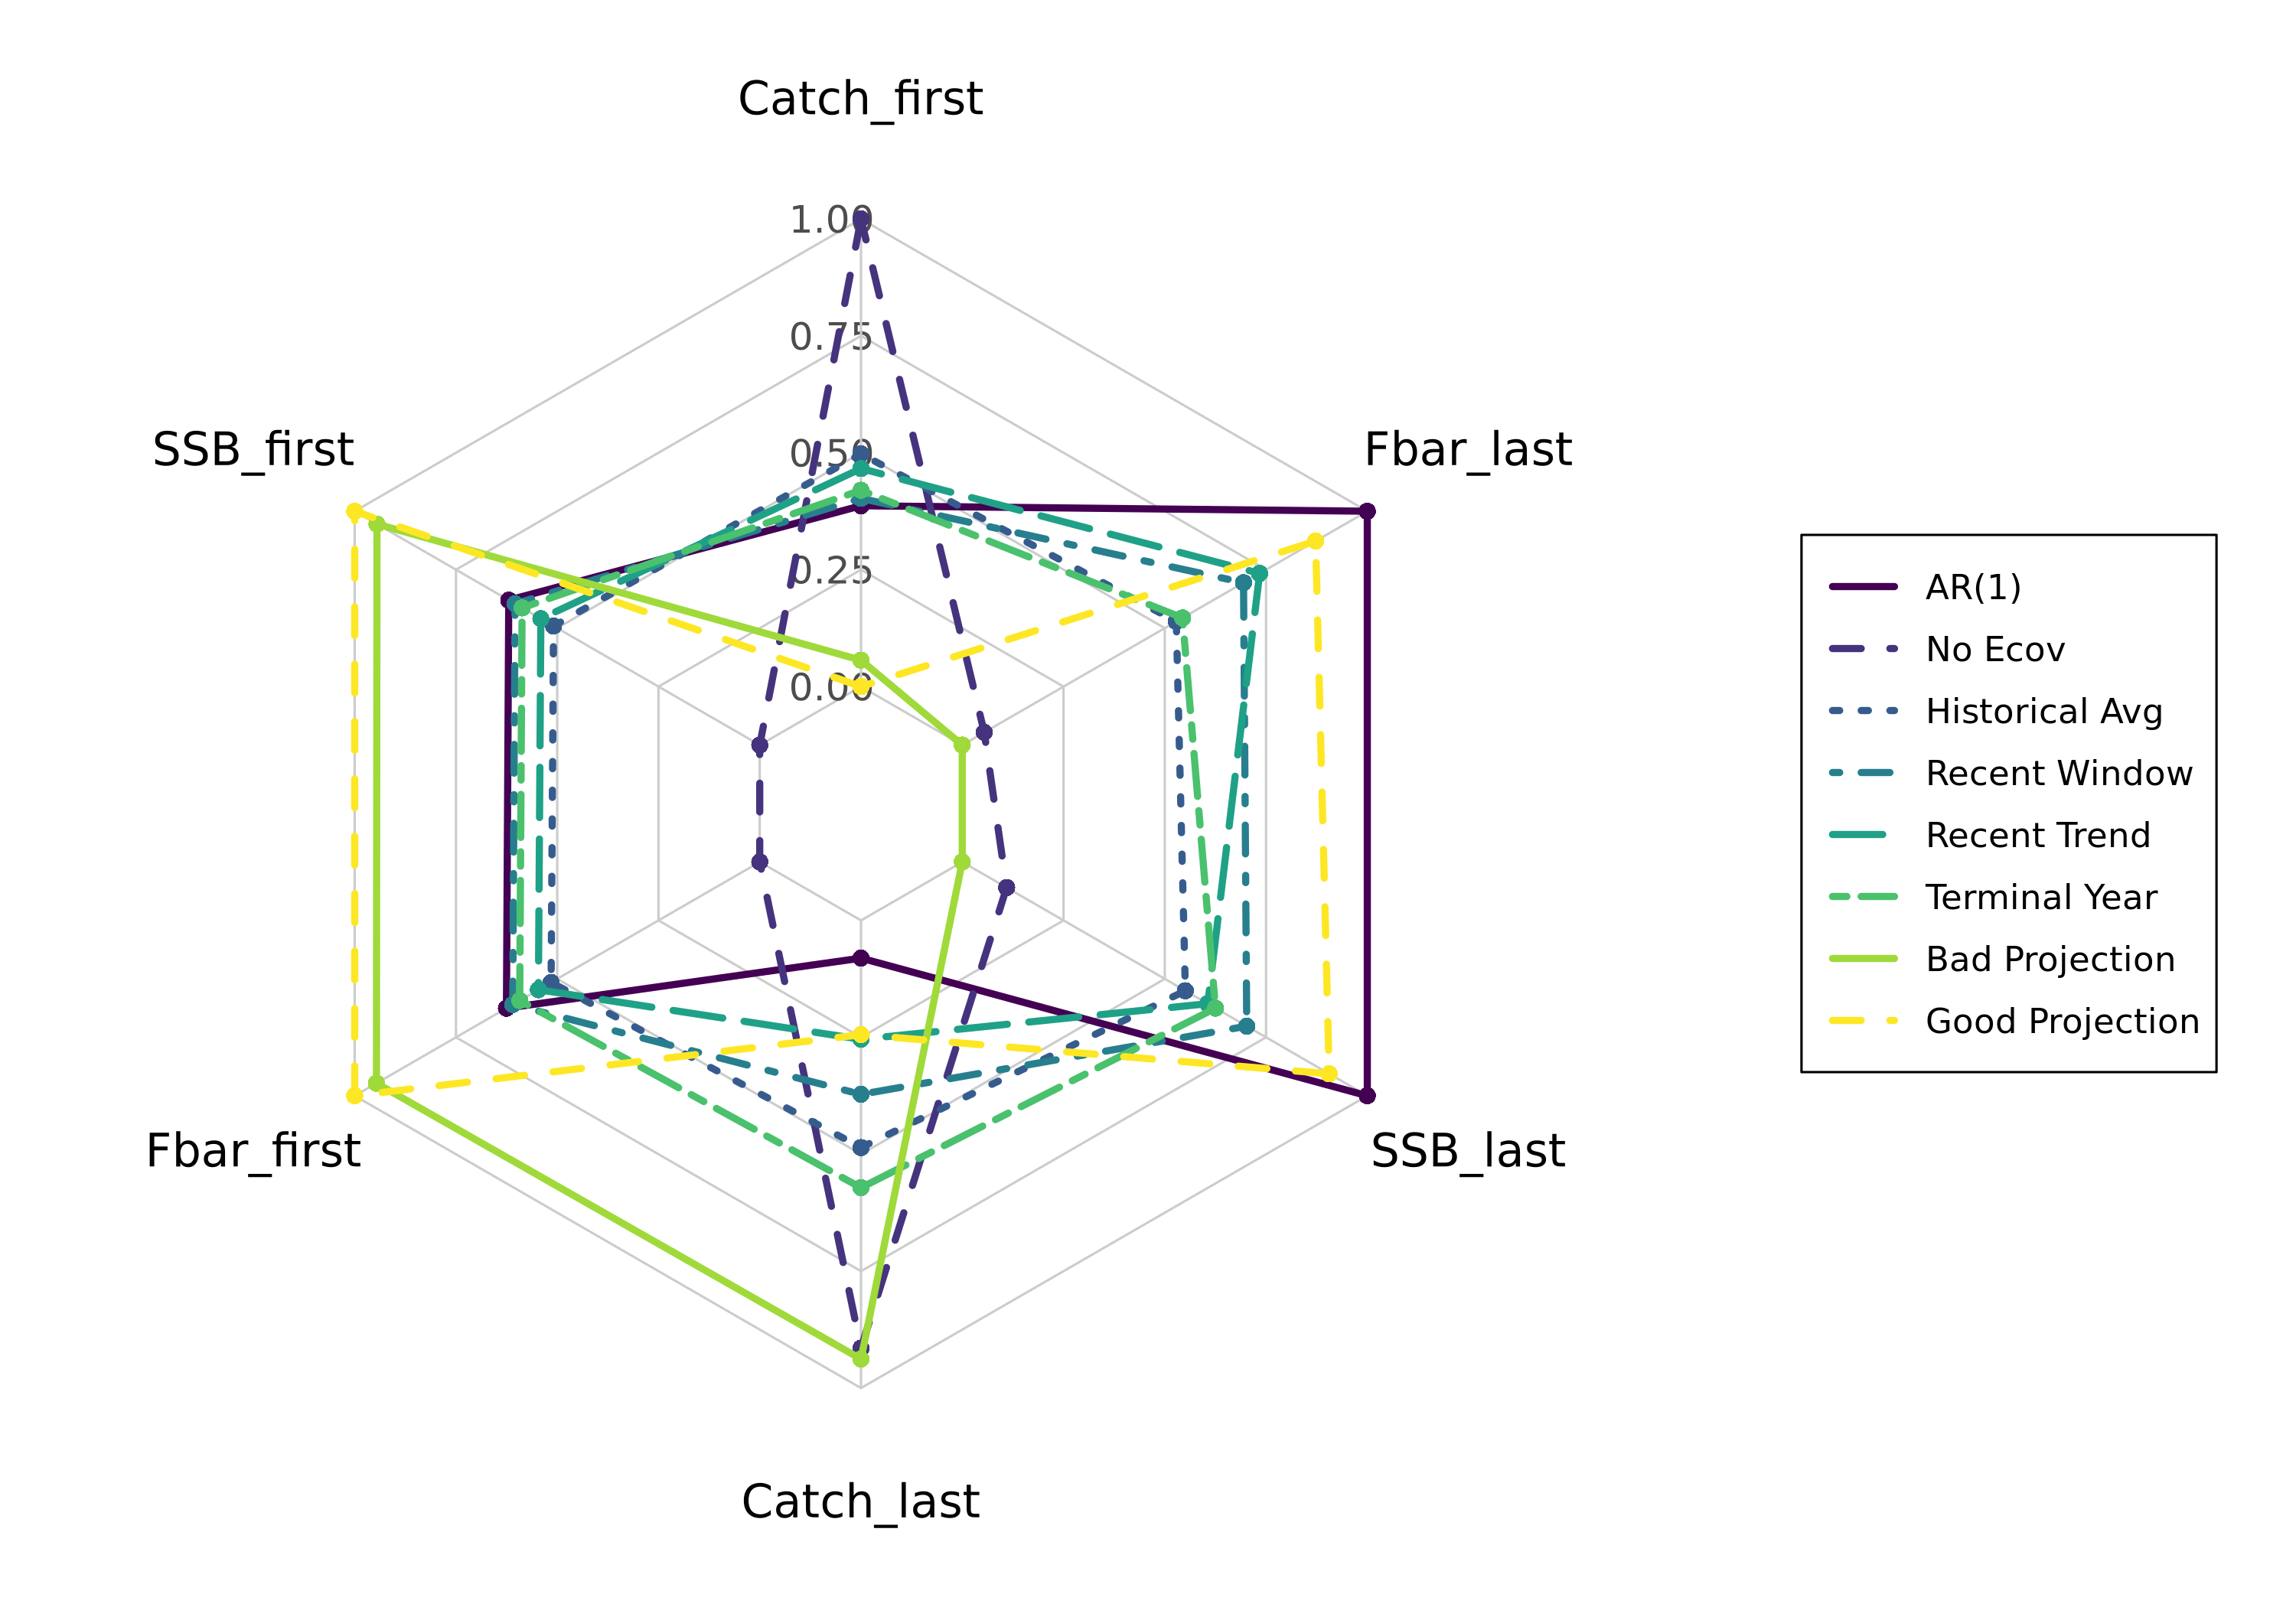
\includegraphics[width=0.75\linewidth]{Plots/Projections_model_performance_radar} \caption{Relative performance of each EM in the beginning and terminal 10 years of the simulation}\label{fig:radar}
\end{figure}

\begin{figure}

{\centering 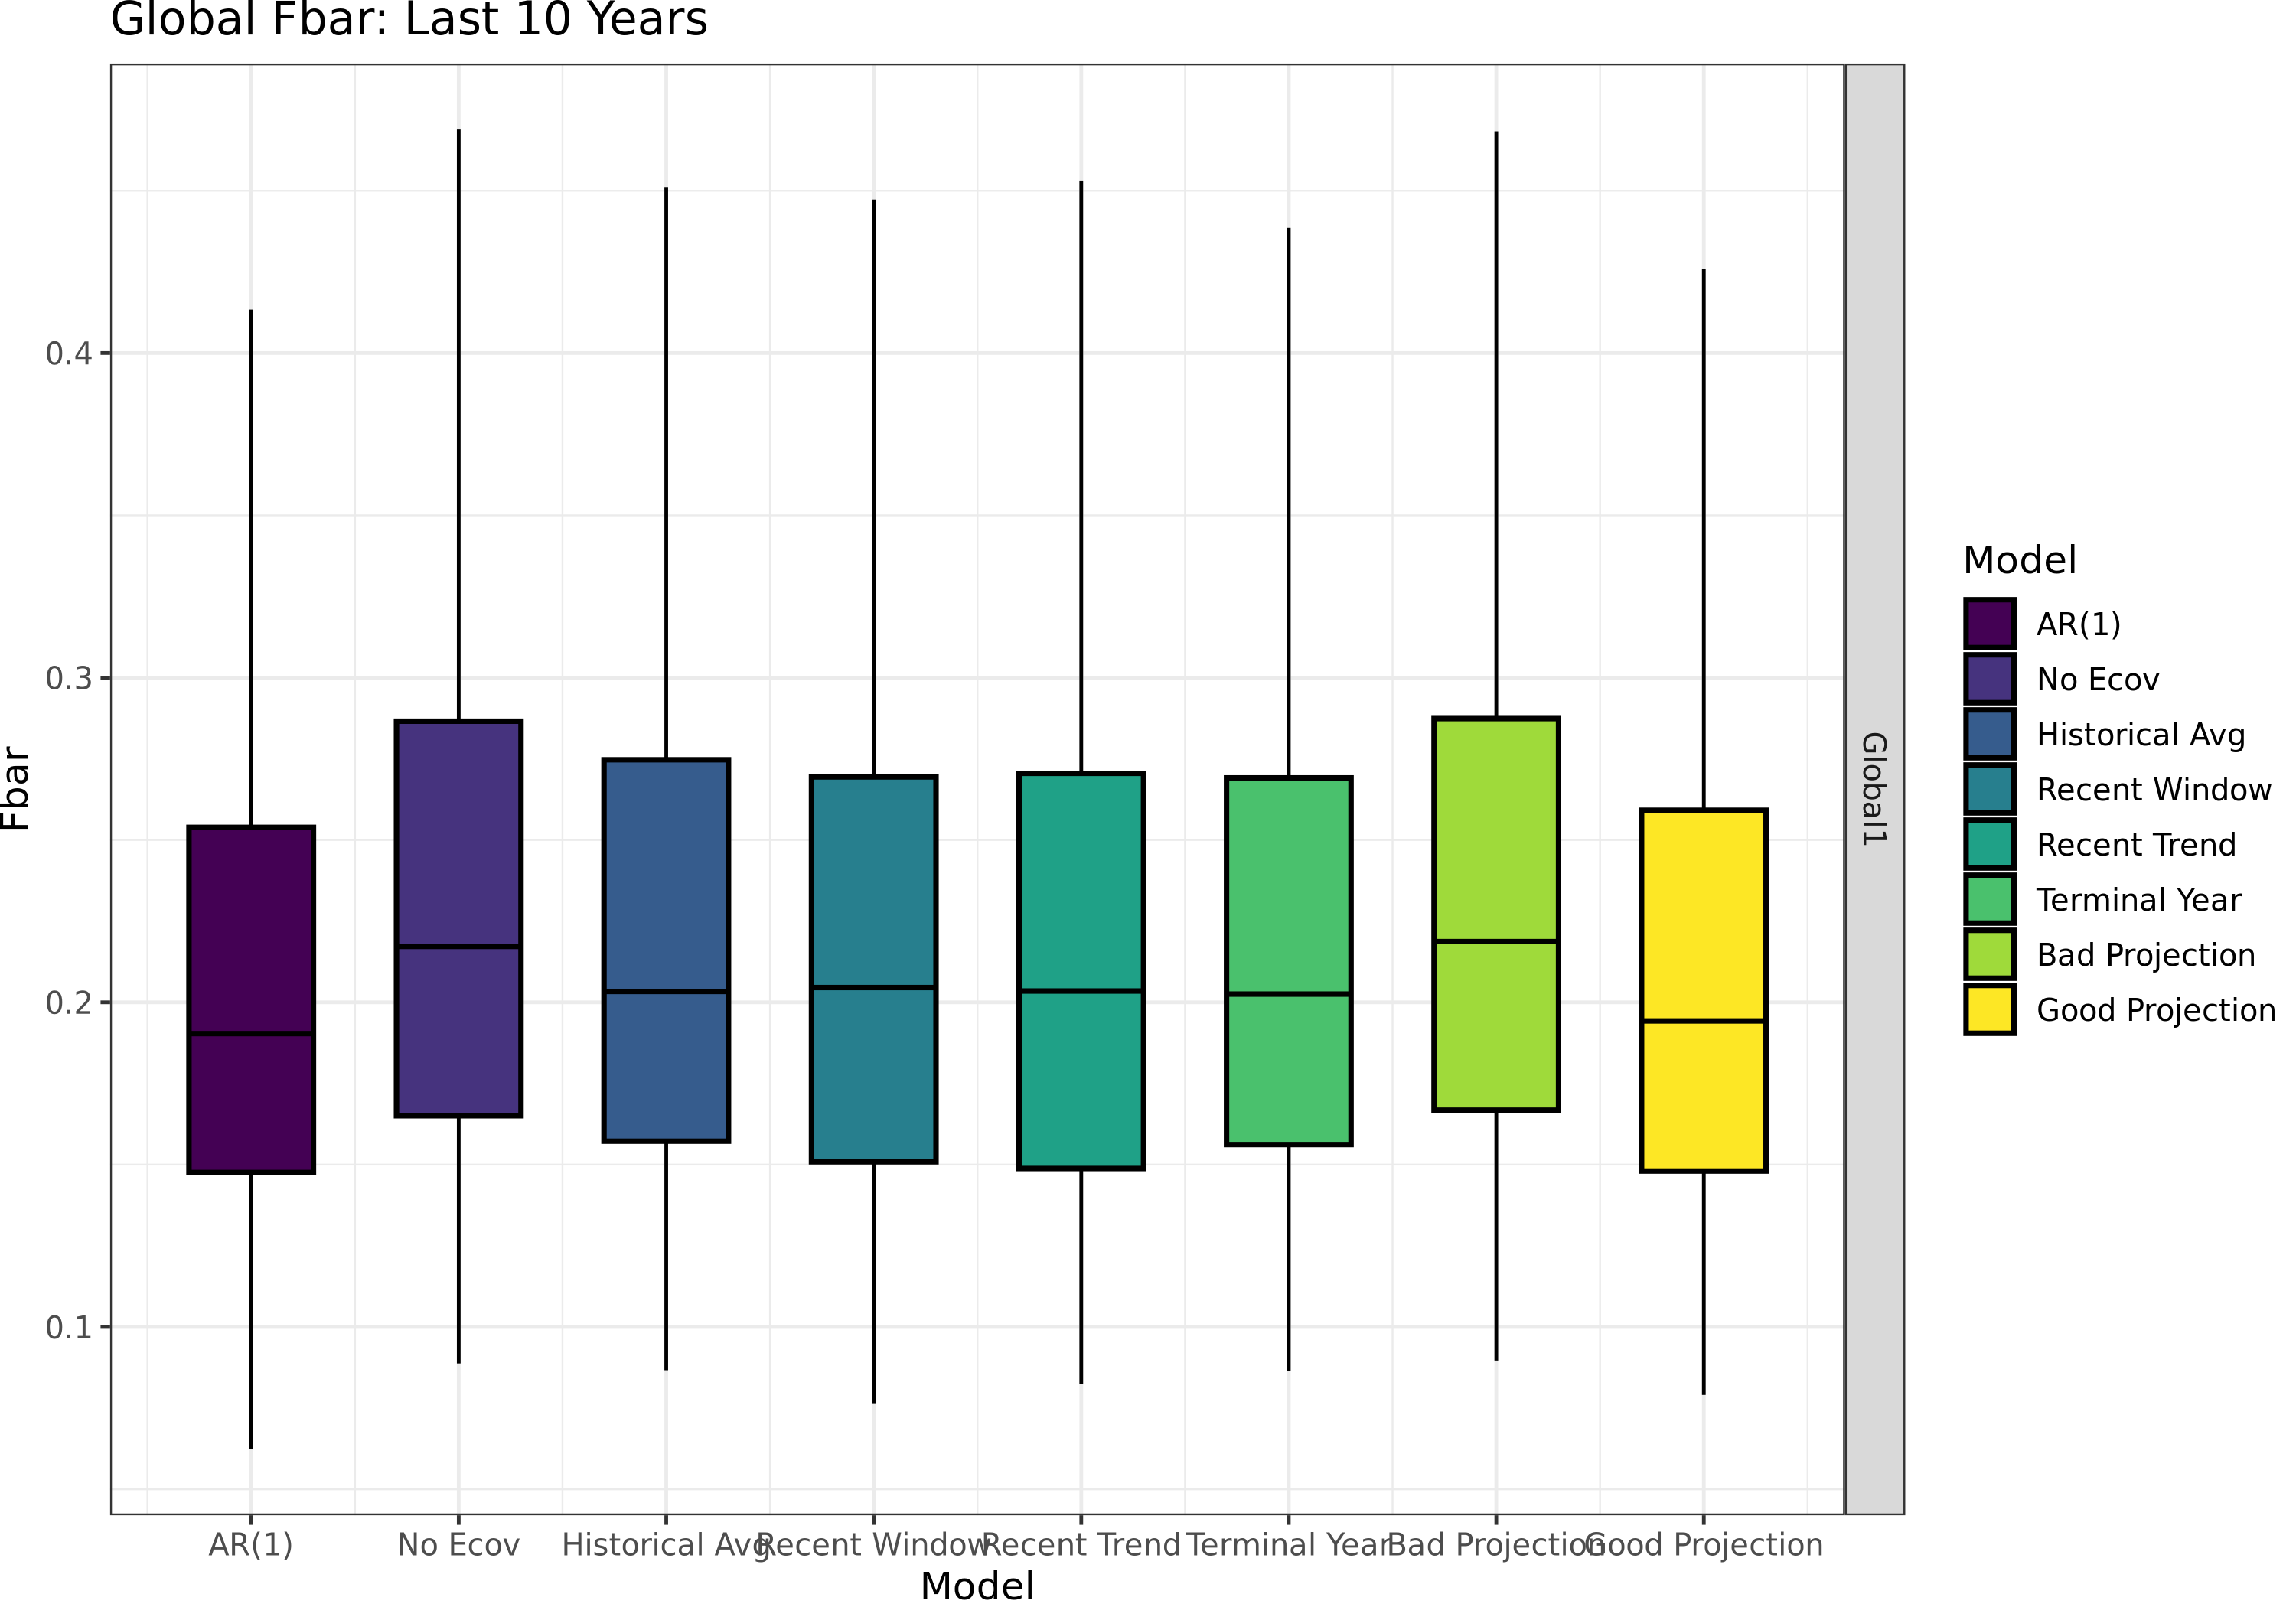
\includegraphics[width=0.3\linewidth]{Plots/Projections_Fbar_global_last_10_years} 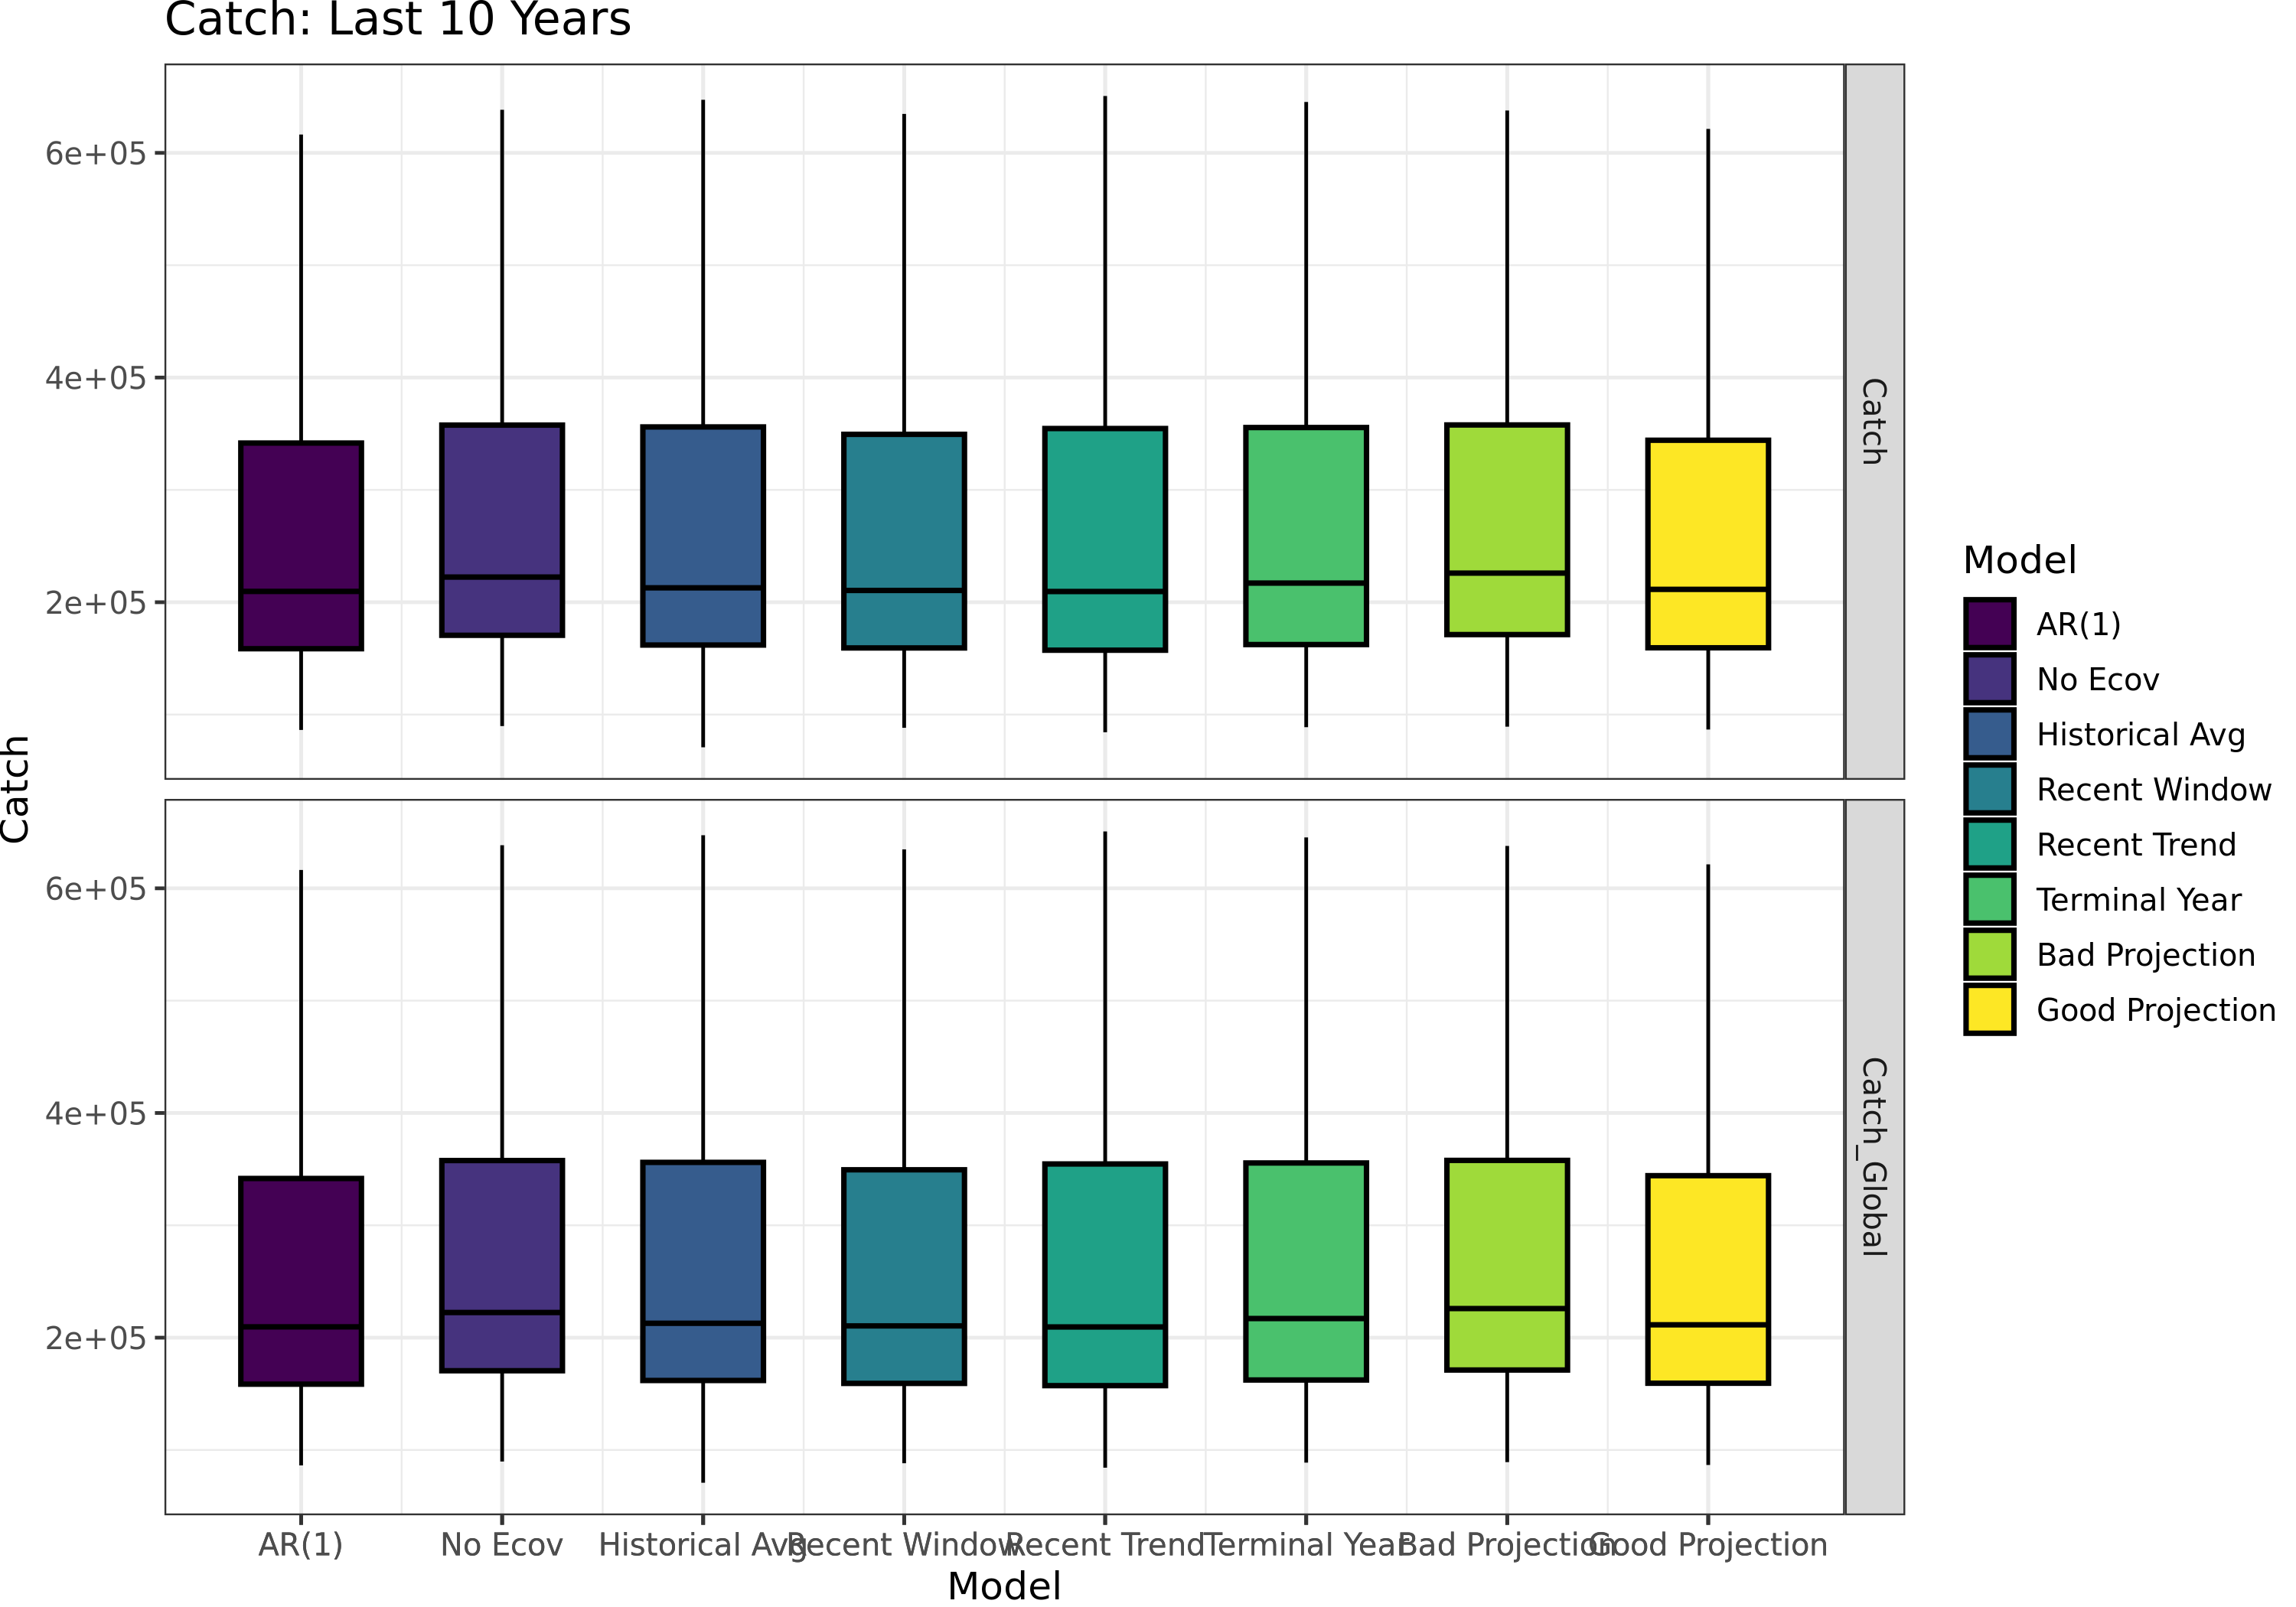
\includegraphics[width=0.3\linewidth]{Plots/Projections_Catch_last_10_years} 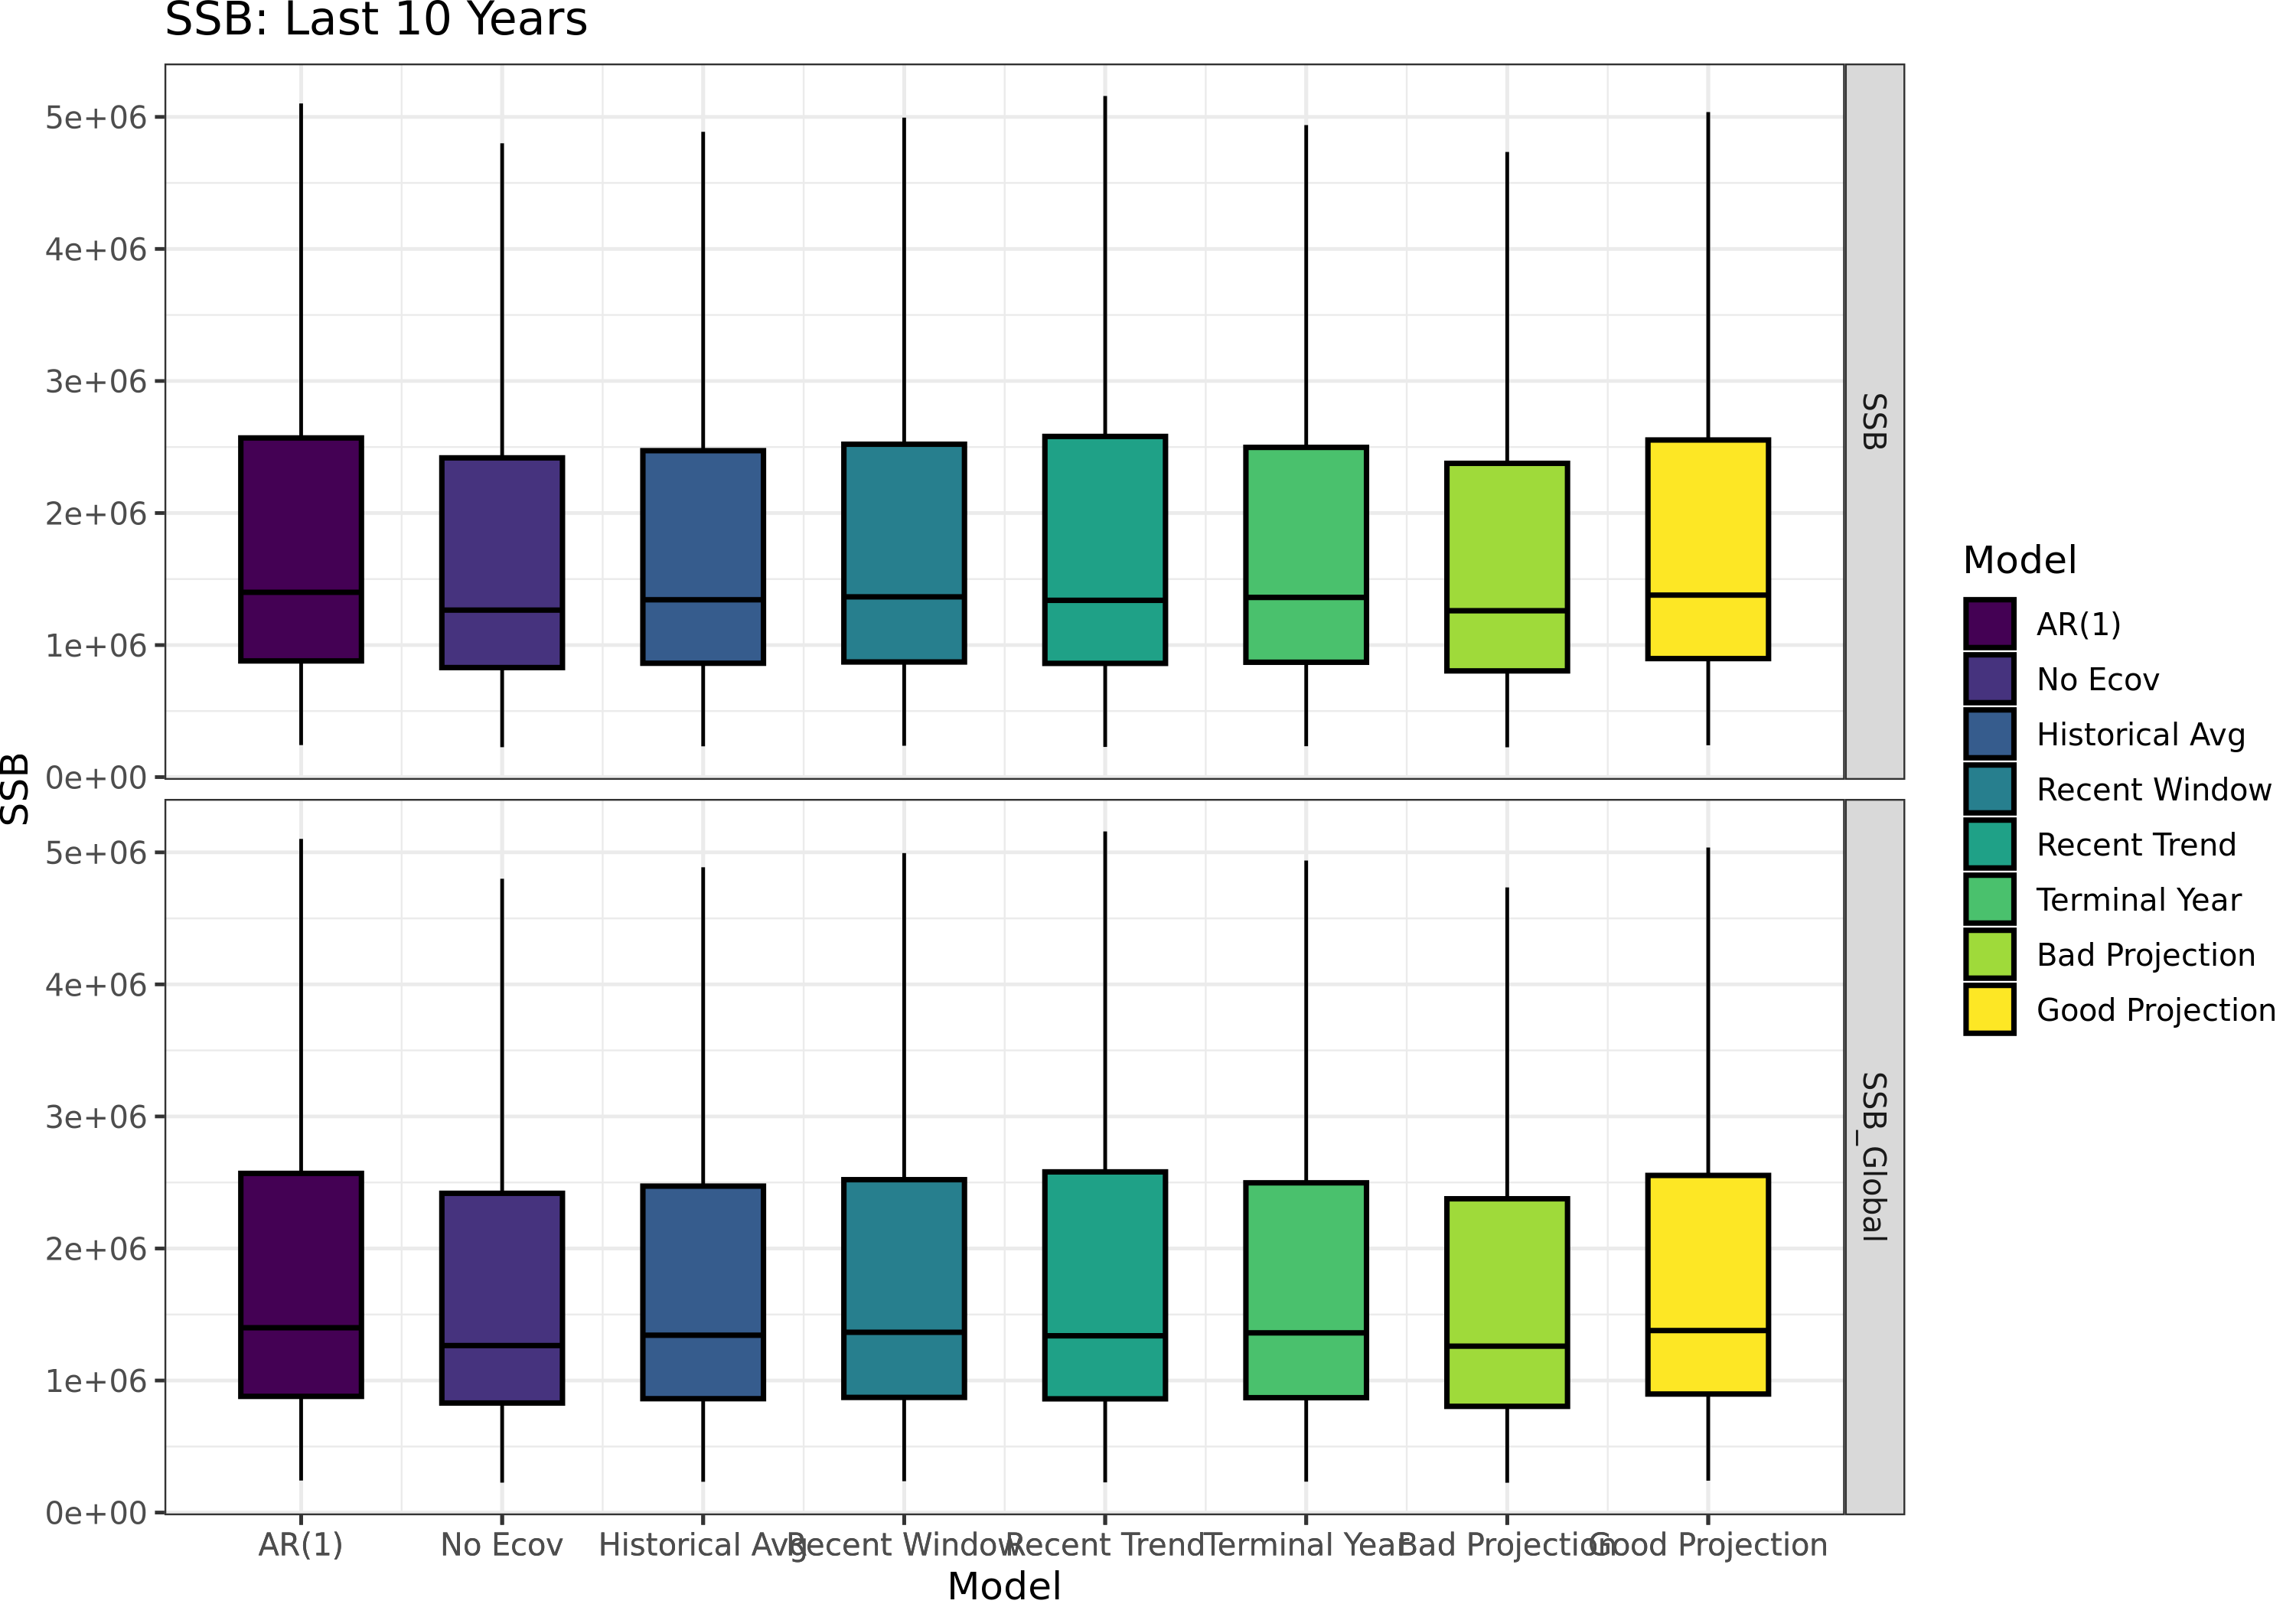
\includegraphics[width=0.3\linewidth]{Plots/Projections_SSB_last_10_years} 

}

\caption{F, SSB, and catch of terminal 10 years of MSE in projections test}\label{fig:projterminal3}
\end{figure}

\begin{figure}
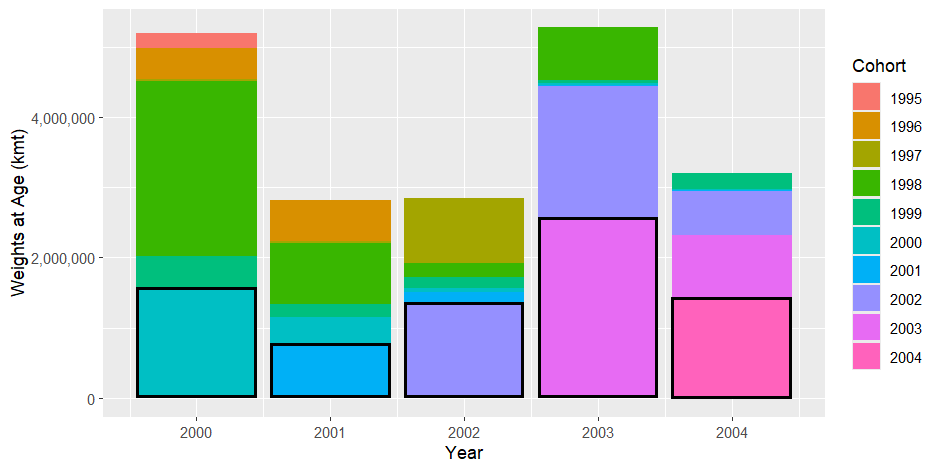
\includegraphics[width=0.75\linewidth]{Plots/CohortAnalysis} \caption{A sub-sample of Weights at Age per year. Each year's cohort is outlined in black}\label{fig:cohortAnalysis}
\end{figure}

\subsection{5-Year Assessment Tests}\label{year-assessment-tests}

When comparing the performance of 5 year assessment periods, a similar pattern emerges as to which projections over or under estimate the true ecological covariate. However in the 5-year assessment period, the performance of the recent window projection is reduced, and this is outperformed by the `bad' climate projection, with only a 2\% average difference between the true covariate and that which was estimated (table \ref{tab:paramEsts5Yr}). This does have notable consequences for the resulting catch advice and estimated \(\bar{F}\) among management periods, with the 5 year period exhibiting much more dramatic `swings' in between periods of high and low predicted catch, mortality, and catch advice, whereas the 3 year management schedule has these oscillations, but with lower amplitudes. SSB is generally under estimated with a reduced management schedule.

\begin{table}

\caption{\label{tab:paramEsts5Yr}Ecov parameter estimates, standard deviation, and rho for each EM for projection}
\centering
\begin{tabular}[t]{l|r|r|r|r}
\hline
EM Name & OM Ecov & Mean Ecov & Percent Change & Ecov Standard Dev.\\
\hline
AR(1) & -0.397 & -0.507 & 27.708 & 0.206\\
\hline
Bad Projection & -0.397 & -0.405 & 2.015 & 0.167\\
\hline
Good Projection & -0.397 & -0.310 & -21.914 & 0.150\\
\hline
Historical Average & -0.397 & -0.541 & 36.272 & 0.243\\
\hline
Recent Trend & -0.397 & -0.325 & -18.136 & 0.142\\
\hline
Recent Window & -0.397 & -0.432 & 8.816 & 0.172\\
\hline
Terminal Year & -0.397 & -0.500 & 25.945 & 0.194\\
\hline
\end{tabular}
\end{table}

\begin{figure}
\centering
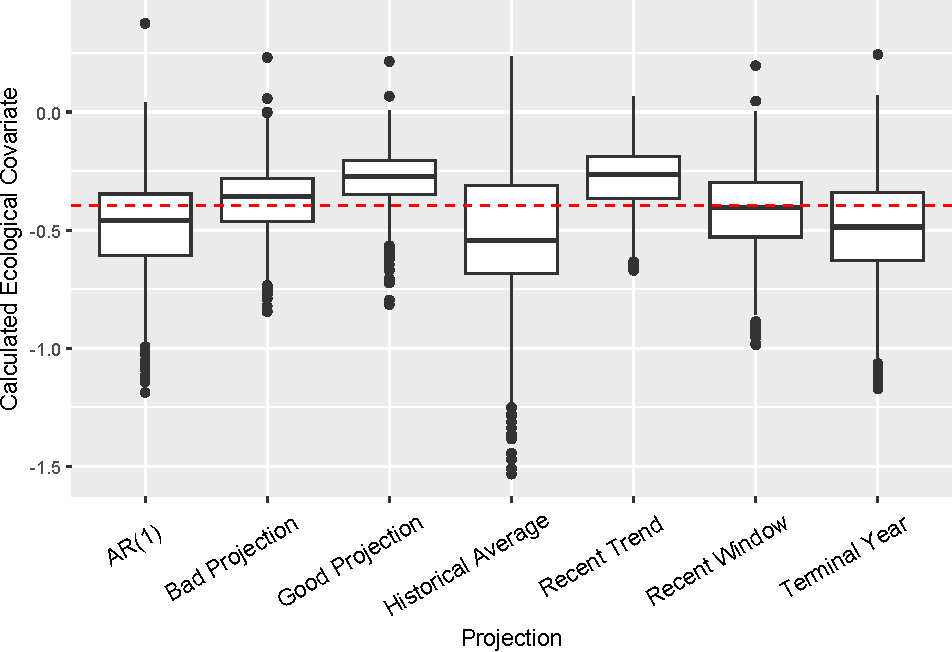
\includegraphics{YT_ProjDraft2_files/figure-latex/paramEsts5Yr-1.pdf}
\caption{\label{fig:paramEsts5Yr}Estimated ecological covariates in for the different biased temperature projections in the EM compared to the ``true'' value in the OM.}
\end{figure}

\begin{figure}
\centering
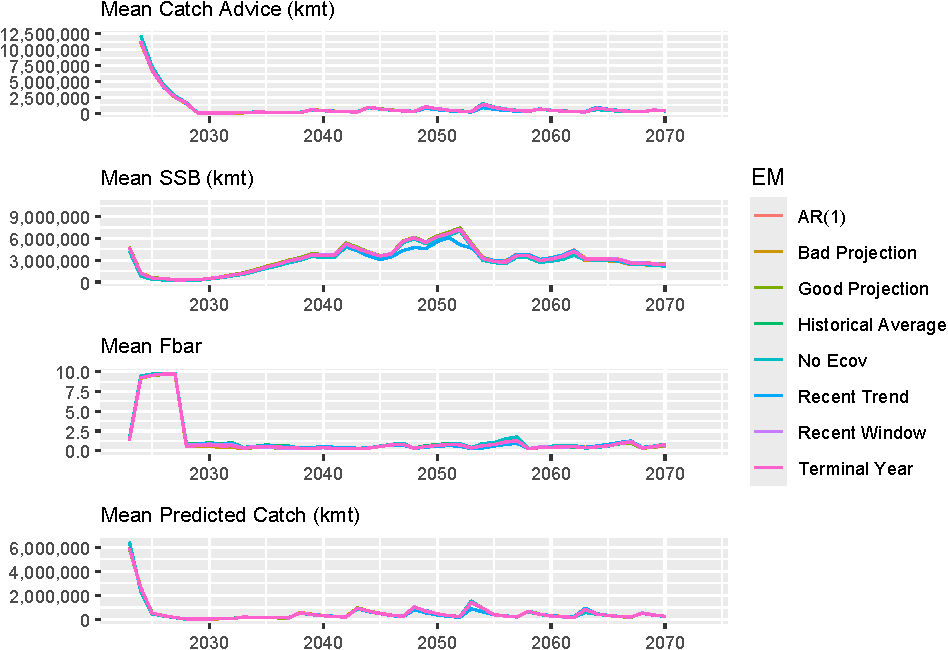
\includegraphics{YT_ProjDraft2_files/figure-latex/timeseries5Yr-1.pdf}
\caption{\label{fig:timeseries5Yr}Catch advice (top), SSB (second), FBar (third), and predicted catch (bottom) calculated from each EM over the projection period}
\end{figure}

Conducting assessments every 5 years increases the amount of variability in recruitment that the ecological covariate accounts for, averaging almost 14\% across simulations and projections (table \ref{tab:recruitmentDevs5Yr}). However this average remained very similar among the different projection choices.

\begin{table}

\caption{\label{tab:recruitmentDevs5Yr}Similar to my other questions, should I combine with other table (this one is looking at 5 year assessment cycles)?}
\centering
\begin{tabular}[t]{l|r|r|r|r}
\hline
EM Name & Mean & SD & Minimum & Maximum\\
\hline
Mod\_AR1Ecov & 13.9285 & 5.7850 & -3.2859 & 28.8318\\
\hline
Mod\_BadProj & 13.9585 & 5.7506 & -3.2503 & 28.9088\\
\hline
Mod\_GoodProj & 13.9448 & 5.7853 & -3.2723 & 28.8877\\
\hline
Mod\_HistAvgEcov & 13.9590 & 5.7916 & -3.2511 & 28.8892\\
\hline
Mod\_RecTrendEcov & 13.9352 & 5.7799 & -3.2945 & 29.4472\\
\hline
Mod\_RecWindEcov & 13.9290 & 5.7934 & -3.2696 & 29.0147\\
\hline
Mod\_TermYear & 13.9604 & 5.7952 & -3.2616 & 28.9537\\
\hline
\end{tabular}
\end{table}

\section{DISCUSSION}\label{discussion}

The results from the bias test show that, while incorporating the ecological covariate helps model performance overall, the trajectory of the projection of temperature used in predicting future simulations will predictably under or over estimate the ecological parameter depending on the type of bias. As a result, low biases tend to under-estimate SSB and higher biases tend to predict higher SSBs. The differences in \(\bar{F}\) across biases becomes greater in warmer climate scenarios. Underestimating the future climate projection could result in highly variable \(\bar{F}\) calculations. However these differences had a limited affect on catch advice and predicted catch. Because warmer `real-world' scenarios supported lower SSB estimations, this means the fishery could risk higher rates of overfishing in warmer climates, with higher \(\bar{F}\) associated with under-estimating this environmental change. Northeast Fisheries Science Center, Woods Hole, MA, USA et al. (2025) found that changing climate conditions have overidden effective management of yellowtail flounder in the early 2000's, and our findings show that these management challenges could persist if bottom temperatures continue to warm quickly. This is contrary to findings from Kell et al. (2005), which found that the specific climate scenario modeled in the OM had a limited affect on the recoverability of Atlantic cod stocks.

However, this test was more of a hypothetical exploration of how diverging temperature projections changes the outputs of the model. In reality, stock assessments use hindcast environmental information, so it is not realistic that an assessment would continue to use a temperature trajectory that diverges away from the real environmental conditions. Instead, stock assessments incorporate the most recent data and use this information to make predictions until the next assessment. This is why our projections test updated its temperature predictions with the previous three years of information. Similar to the bias tests, we found that incorporating the environmental covariate resulted in slightly different dynamics, but overall followed similar trajectories. Some models appeared to do better with some metrics (e.g.~recent window projections resulted in the most accurate ecological covariate), but this had a limited impact in the overall fishery dynamics, even in the long term. This is in line with previous literature for yellowtail flounder, which has shown that there is little discernible difference between projections that used a continued estimated environmental process, ones that fixed the environmental process at recent 5 year average, and a third EM which used the observed environmental index (Britten et al., 2024) ADD ALEX. This research also noted that the specific stock-recruitment relationship defined in the model will change the environmental affect size due to the placement of the environmental covariate in the stock-recruit equation. McClatchie et al. (2010) found that for Pacific sardine, \emph{Sardinops sagax}, temperature actually did not have a relationship with recruitment, and the correlation between temperature parameters and recruitment depended on the amount of autocorrelation in the temperature time series, although the specific mechanism that links Pacific sardine recruitment is less clear than with yellowtail flounder. This may also be due to the amount of recruitment variation that was explained by the ecological covariate. In these simulations, the percentage of variation explained by the ecological covariate had a maximum of 25.47\% in one simulation, yet De Oliveira \& Butterworth (2005) found that management strategies do not show any benefits to risk and average catch if the ecological covariate explains less than 50\% of recruitment variation. None of the simulations in this experiment exceeded 50\%.

This could be the result of the type of link that the environmental covariate makes with the population. For Georges Bank Yellowtail, the environmental covariate has a lagged controlling effect on recruitment (CITE RT). Over time, the negative effects of high temperature could be masked by density-dependent mortality, or other factors that occur during the lag. Kell et al. (2005) found that the long-term performance and calculated reference points of Atlantic cod stock depended on if ocean temperatures were linked to juvenile survival versus the carrying capacity of the stock. Further, there may be a greater difference in model outputs if the environmental covariate had a direct effect on distribution, carrying capacity, catchability, mortality, behavioral, migratory, spawning, or metabolic processes; life history traits that can all be affected by environmental change (Punt et al., 2014; Stock \& Miller, 2021), indicating a need for further research on projection choices for environmental covariates that affect other parts of life history. Catch advice is not very dependent on recruitment, and because this environmental link is also lagged, these combined factors could be masking the effect. Further, Haltuch \& Punt (2011) has shown that incorrectly including environmental covariates in the stock does not have a large effect on biomass reference points or relative errors of the model. A review by Punt et al. (2014) has also shown that short and medium-term fisheries management simulations are generally not greatly improved by incorporating environmental covariates. This research served to test a longer-term simulation and found a similar result. However, if there is a high temporal contrast in the `real world' or OM, incorporating the environmental covariate in the estimation model can improve model accuracy (Miller et al., 2023). This could indicate that these results may change depending on the amount of future variation in ocean bottom temperatures.

Instead of projection choices influencing model dynamics, changing from a 3-year to a 5-year assessment period had a larger affect on the simulated catch advice and \(\bar{F}\). This result implies that the choice of projection will still produce similar results, but this transition to the less frequent schedule could have repercussions on the stability of the fishery, with larger swings in between periods of high SSB and catch and periods of low stocks and strict management measures.

Future ocean conditions are expected to be highly variable in coming years due to climate change, (Wang et al., 2010), so understanding potential impacts on fishery dynamics is vital. Overall, we found that projection decisions had a limited effect on catch advice and fishery dynamics in an MSE framework and other model components, such as assessment frequency and recruitment variation, had a larger influence on catch and management advice. This could be due to the nature of the environmental link to Georges Bank Yellowtail flounder, indicating a need for further research on how this type of link will affect model dynamics over different projection decisions.

\newpage

\textbf{References}

\phantomsection\label{refs}
\begin{CSLReferences}{1}{2}
\bibitem[\citeproctext]{ref-abraham2013}
Abraham, J. P., Baringer, M., Bindoff, N. L., Boyer, T., Cheng, L. J., Church, J. A., Conroy, J. L., Domingues, C. M., Fasullo, J. T., Gilson, J., Goni, G., Good, S. A., Gorman, J. M., Gouretski, V., Ishii, M., Johnson, G. C., Kizu, S., Lyman, J. M., Macdonald, A. M., \ldots{} Willis, J. K. (2013). A review of global ocean temperature observations: Implications for ocean heat content estimates and climate change. \emph{Reviews of Geophysics}, \emph{51}(3), 450--483. \url{https://doi.org/10.1002/rog.20022}

\bibitem[\citeproctext]{ref-albouy2014}
Albouy, C., Velez, L., Coll, M., Colloca, F., Le Loc'h, F., Mouillot, D., \& Gravel, D. (2014). From projected species distribution to food{-}web structure under climate change. \emph{Global Change Biology}, \emph{20}(3), 730--741. \url{https://doi.org/10.1111/gcb.12467}

\bibitem[\citeproctext]{ref-brittenIdentificationPerformanceStockrecruitment2024}
Britten, G. L., Brooks, E., \& Miller, T. (2024). \emph{Identification and performance of stock-recruitment functions in state space assessment models}. NEFSC.

\bibitem[\citeproctext]{ref-buckley2004}
Buckley, L. J., Caldarone, E. M., \& Lough, R. G. (2004). Optimum temperature and food{-}limited growth of larval Atlantic cod ( {\emph{Gadus morhua}} ) and haddock ( {\emph{Melanogrammus aeglefinus}} ) on Georges Bank. \emph{Fisheries Oceanography}, \emph{13}(2), 134--140. \url{https://doi.org/10.1046/j.1365-2419.2003.00278.x}

\bibitem[\citeproctext]{ref-chaikin2024}
Chaikin, S., Riva, F., Marshall, K. E., Lessard, J.-P., \& Belmaker, J. (2024). Marine fishes experiencing high-velocity range shifts may not be climate change winners. \emph{Nature Ecology \& Evolution}, \emph{8}(5), 936--946. \url{https://doi.org/10.1038/s41559-024-02350-7}

\bibitem[\citeproctext]{ref-cheng2024}
Cheng, L., Abraham, J., Trenberth, K. E., Boyer, T., Mann, M. E., Zhu, J., Wang, F., Yu, F., Locarnini, R., Fasullo, J., Zheng, F., Li, Y., Zhang, B., Wan, L., Chen, X., Wang, D., Feng, L., Song, X., Liu, Y., \ldots{} Lu, Y. (2024). New Record Ocean Temperatures and Related Climate Indicators in 2023. \emph{Advances in Atmospheric Sciences}, \emph{41}(6), 1068--1082. \url{https://doi.org/10.1007/s00376-024-3378-5}

\bibitem[\citeproctext]{ref-chown2010}
Chown, S., Hoffmann, A., Kristensen, T., Angilletta, M., Stenseth, N., \& Pertoldi, C. (2010). Adapting to climate change: a perspective from evolutionary physiology. \emph{Climate Research}, \emph{43}(1), 3--15. \url{https://doi.org/10.3354/cr00879}

\bibitem[\citeproctext]{ref-CurrentStockAssessment2026}
Current {Stock Assessment Schedules}. (2026). In \emph{New England Fishery Management Council}.

\bibitem[\citeproctext]{ref-deoliveiraLimitsUseEnvironmental2005}
De Oliveira, J., \& Butterworth, D. (2005). Limits to the use of environmental indices to reduce risk and/or increase yield in the {South African} anchovy fishery. \emph{African Journal of Marine Science}, \emph{27}(1), 191--203. \url{https://doi.org/10.2989/18142320509504078}

\bibitem[\citeproctext]{ref-dupontavice2023}
Du Pontavice, H., Chen, Z., \& Saba, V. S. (2023). A high-resolution ocean bottom temperature product for the northeast U.S. continental shelf marine ecosystem. \emph{Progress in Oceanography}, \emph{210}, 102948. \url{https://doi.org/10.1016/j.pocean.2022.102948}

\bibitem[\citeproctext]{ref-ehrluxe9n2015}
Ehrlén, J., \& Morris, W. F. (2015). Predicting changes in the distribution and abundance of species under environmental change. \emph{Ecology Letters}, \emph{18}(3), 303--314. \url{https://doi.org/10.1111/ele.12410}

\bibitem[\citeproctext]{ref-fabry2008}
Fabry, V. J., Seibel, B. A., Feely, R. A., \& Orr, J. C. (2008). Impacts of ocean acidification on marine fauna and ecosystem processes. \emph{ICES Journal of Marine Science}, \emph{65}(3), 414--432. \url{https://doi.org/10.1093/icesjms/fsn048}

\bibitem[\citeproctext]{ref-friedland2022}
Friedland, K. D., Miles, T., Goode, A. G., Powell, E. N., \& Brady, D. C. (2022). The Middle Atlantic Bight Cold Pool is warming and shrinking: Indices from in situ autumn seafloor temperatures. \emph{Fisheries Oceanography}, \emph{31}(2), 217--223. \url{https://doi.org/10.1111/fog.12573}

\bibitem[\citeproctext]{ref-fulton2021}
Fulton, E. A. (2021). Opportunities to improve ecosystem{-}based fisheries management by recognizing and overcoming path dependency and cognitive bias. \emph{Fish and Fisheries}, \emph{22}(2), 428--448. \url{https://doi.org/10.1111/faf.12537}

\bibitem[\citeproctext]{ref-garcuxedamolinos2017}
García Molinos, J., Burrows, M. T., \& Poloczanska, E. S. (2017). Ocean currents modify the coupling between climate change and biogeographical shifts. \emph{Scientific Reports}, \emph{7}(1), 1332. \url{https://doi.org/10.1038/s41598-017-01309-y}

\bibitem[\citeproctext]{ref-guinotte2008}
Guinotte, J. M., \& Fabry, V. J. (2008). Ocean Acidification and Its Potential Effects on Marine Ecosystems. \emph{Annals of the New York Academy of Sciences}, \emph{1134}(1), 320--342. \url{https://doi.org/10.1196/annals.1439.013}

\bibitem[\citeproctext]{ref-haltuchPromisesPitfallsIncluding2011}
Haltuch, M. A., \& Punt, A. E. (2011). The promises and pitfalls of including decadal-scale climate forcing of recruitment in groundfish stock assessment. \emph{Canadian Journal of Fisheries and Aquatic Sciences}, \emph{68}(5), 912--926. \url{https://doi.org/10.1139/f2011-030}

\bibitem[\citeproctext]{ref-hare2016}
Hare, J. A., Morrison, W. E., Nelson, M. W., Stachura, M. M., Teeters, E. J., Griffis, R. B., Alexander, M. A., Scott, J. D., Alade, L., Bell, R. J., Chute, A. S., Curti, K. L., Curtis, T. H., Kircheis, D., Kocik, J. F., Lucey, S. M., McCandless, C. T., Milke, L. M., Richardson, D. E., \ldots{} Griswold, C. A. (2016). A Vulnerability Assessment of Fish and Invertebrates to Climate Change on the Northeast U.S. Continental Shelf. \emph{PLOS ONE}, \emph{11}(2), e0146756. \url{https://doi.org/10.1371/journal.pone.0146756}

\bibitem[\citeproctext]{ref-hobday2016}
Hobday, A. J., Spillman, C. M., Paige Eveson, J., \& Hartog, J. R. (2016). Seasonal forecasting for decision support in marine fisheries and aquaculture. \emph{Fisheries Oceanography}, \emph{25}(S1), 45--56. \url{https://doi.org/10.1111/fog.12083}

\bibitem[\citeproctext]{ref-hollowed2011}
Hollowed, A., A'mar, T., Barbeaux, S., Bond, N., Ianelli, J., Spncer, P., \& Wilderbuer, T. (2011). \emph{Integrating Ecosystem Aspects and Climate Change Forecasting into Stock Assessments}.

\bibitem[\citeproctext]{ref-honischGeologicalRecordOcean2012}
Hönisch, B., Ridgwell, A., Schmidt, D. N., Thomas, E., Gibbs, S. J., Sluijs, A., Zeebe, R., Kump, L., Martindale, R. C., Greene, S. E., Kiessling, W., Ries, J., Zachos, J. C., Royer, D. L., Barker, S., Marchitto, T. M., Moyer, R., Pelejero, C., Ziveri, P., \ldots{} Williams, B. (2012). The {Geological Record} of {Ocean Acidification}. \emph{Science}, \emph{335}(6072), 1058--1063. \url{https://doi.org/10.1126/science.1208277}

\bibitem[\citeproctext]{ref-hyun2014}
Hyun, S.-Y., Cadrin, S. X., \& Roman, S. (2014). Fixed and mixed effect models for fishery data on depth distribution of Georges Bank yellowtail flounder. \emph{Fisheries Research}, \emph{157}, 180--186. \url{https://doi.org/10.1016/j.fishres.2014.04.010}

\bibitem[\citeproctext]{ref-johnsonYellowtailFlounderLimanda1999}
Johnson, D., Morse, W., Berrien, P., \& Vitaliano, J. (1999). \emph{Yellowtail {Flounder}, {Limanda} ferruginea, {Life History} and {Habitat Characteristics}} (NOAA Technical Memorandum NMFS-NE-140). US Department of Commerce.

\bibitem[\citeproctext]{ref-kellImplicationsClimateChange2005}
Kell, L. T., Pilling, G. M., \& O'Brien, C. M. (2005). Implications of climate change for the management of {North Sea} cod ({Gadus} morhua). \emph{ICES Journal of Marine Science}, \emph{62}(7), 1483--1491. \url{https://doi.org/10.1016/j.icesjms.2005.05.006}

\bibitem[\citeproctext]{ref-kerr2022}
Kerr, L., Barajas, M., \& Wiedenmann, J. (2022). Coherence and potential drivers of stock assessment uncertainty in Northeast US groundfish stocks. \emph{ICES Journal of Marine Science}, \emph{79}(8), 2217--2230. \url{https://doi.org/10.1093/icesjms/fsac140}

\bibitem[\citeproctext]{ref-klein2017}
Klein, E. S., Smith, S. L., \& Kritzer, J. P. (2017). Effects of climate change on four New England groundfish species. \emph{Reviews in Fish Biology and Fisheries}, \emph{27}(2), 317--338. \url{https://doi.org/10.1007/s11160-016-9444-z}

\bibitem[\citeproctext]{ref-kleisner2017}
Kleisner, K. M., Fogarty, M. J., McGee, S., Hare, J. A., Moret, S., Perretti, C. T., \& Saba, V. S. (2017). Marine species distribution shifts on the U.S. Northeast Continental Shelf under continued ocean warming. \emph{Progress in Oceanography}, \emph{153}, 24--36. \url{https://doi.org/10.1016/j.pocean.2017.04.001}

\bibitem[\citeproctext]{ref-laurence1981}
Laurence, G., \& Howell, W. H. (1981). Embryology and influence of temperature and salinity on early development and survival of yellowtail flounder limanda ferruginea. \emph{Marine Ecology Progress Series}, \emph{6}, 11--18.

\bibitem[\citeproctext]{ref-mazur2023}
Mazur, M. D., Jesse, J., Cadrin, S. X., Truesdell, S. B., \& Kerr, L. (2023). Consequences of ignoring climate impacts on New England groundfish stock assessment and management. \emph{Fisheries Research}, \emph{262}, 106652. \url{https://doi.org/10.1016/j.fishres.2023.106652}

\bibitem[\citeproctext]{ref-mcclatchieReassessmentStockRecruit2010}
McClatchie, S., Goericke, R., Auad, G., \& Hill, K. (2010). Re-assessment of the stock--recruit and temperature--recruit relationships for {Pacific} sardine ({Sardinops} sagax). \emph{Canadian Journal of Fisheries and Aquatic Sciences}, \emph{67}(11), 1782--1790. \url{https://doi.org/10.1139/F10-101}

\bibitem[\citeproctext]{ref-millerFactorsAffectingInferences2023}
Miller, T. J., Applegate, A., Britten, G., Brooks, E. N., Fay, G., Hansell, A., Legault, C. M., Muffley, B., Stock, B. C., \& Wiedenmann, J. (2023). \emph{Factors affecting inferences on natural mortality and associated environmental effects} {[}Research \{\{Track\}\}{]}. NEFSC.

\bibitem[\citeproctext]{ref-murawski1993}
Murawski, S. A. (1993). Climate Change and Marine Fish Distributions: Forecasting from Historical Analogy. \emph{Transactions of the American Fisheries Society}, \emph{122}(5), 647--658. \url{https://doi.org/10.1577/1548-8659(1993)122\%3C0647:CCAMFD\%3E2.3.CO;2}

\bibitem[\citeproctext]{ref-northeastfisheriessciencecenterwoodsholemausaCollapseRecoveryCollapse2025}
Northeast Fisheries Science Center, Woods Hole, MA, USA, Hansell, A., Barrett, M., Fisheries and Oceans Canada, St. Andrews, NB, Canada, Cadrin, S., University of Massachusetts Dartmouth, School for Marine Science and Technology, New Bedford MA, USA, Carrano, C., University of Massachusetts Dartmouth, School for Marine Science and Technology, New Bedford MA, USA, Kittel, J., Legault, C., \& Northeast Fisheries Science Center, Woods Hole, MA, USA. (2025). Collapse, recovery and collapse of an important fishery. \emph{Journal of Northwest Atlantic Fishery Science}, \emph{56}, 31--46. \url{https://doi.org/10.2960/J.v56.m752}

\bibitem[\citeproctext]{ref-nye2009}
Nye, J., Link, J., Hare, J., \& Overholtz, W. (2009). Changing spatial distribution of fish stocks in relation to climate and population size on the Northeast United States continental shelf. \emph{Marine Ecology Progress Series}, \emph{393}, 111--129. \url{https://doi.org/10.3354/meps08220}

\bibitem[\citeproctext]{ref-overholtz2011}
Overholtz, W. J., Hare, J. A., \& Keith, C. M. (2011). Impacts of Interannual Environmental Forcing and Climate Change on the Distribution of Atlantic Mackerel on the U.S. Northeast Continental Shelf. \emph{Marine and Coastal Fisheries}, \emph{3}(1), 219--232. \url{https://doi.org/10.1080/19425120.2011.578485}

\bibitem[\citeproctext]{ref-poloczanska2016}
Poloczanska, E. S., Burrows, M. T., Brown, C. J., García Molinos, J., Halpern, B. S., Hoegh-Guldberg, O., Kappel, C. V., Moore, P. J., Richardson, A. J., Schoeman, D. S., \& Sydeman, W. J. (2016). Responses of Marine Organisms to Climate Change across Oceans. \emph{Frontiers in Marine Science}, \emph{3}. \url{https://doi.org/10.3389/fmars.2016.00062}

\bibitem[\citeproctext]{ref-puntFisheriesManagementClimate2014}
Punt, A. E., A'mar, T., Bond, N. A., Butterworth, D. S., De Moor, C. L., De Oliveira, J. A. A., Haltuch, M. A., Hollowed, A. B., \& Szuwalski, C. (2014). Fisheries management under climate and environmental uncertainty: Control rules and performance simulation. \emph{ICES Journal of Marine Science}, \emph{71}(8), 2208--2220. \url{https://doi.org/10.1093/icesjms/fst057}

\bibitem[\citeproctext]{ref-punt2016}
Punt, A. E., Butterworth, D. S., De Moor, C. L., De Oliveira, J. A. A., \& Haddon, M. (2016). Management strategy evaluation: best practices. \emph{Fish and Fisheries}, \emph{17}(2), 303--334. \url{https://doi.org/10.1111/faf.12104}

\bibitem[\citeproctext]{ref-saba2016}
Saba, V. S., Griffies, S. M., Anderson, W. G., Winton, M., Alexander, M. A., Delworth, T. L., Hare, J. A., Harrison, M. J., Rosati, A., Vecchi, G. A., \& Zhang, R. (2016). Enhanced warming of the Northwest Atlantic Ocean under climate change. \emph{Journal of Geophysical Research: Oceans}, \emph{121}(1), 118--132. \url{https://doi.org/10.1002/2015JC011346}

\bibitem[\citeproctext]{ref-saba2023}
Saba, V., Borggaard, D., Caracappa, J. C., Chambers, R. C., Clay, P. M., Colburn, L. L., Deroba, J., DePiper, G., Du Pontavice, H., Fratantoni, P., Ferguson, M., Gaichas, S., Hayes, S., Hyde, K., Johnson, M., Kocik, J., Keane, E., Kircheis, D., Large, S., \ldots{} Wikfors, G. (2023). NOAA fisheries research geared towards climate-ready living marine resource management in the northeast United States. \emph{PLOS Climate}, \emph{2}(12), e0000323. \url{https://doi.org/10.1371/journal.pclm.0000323}

\bibitem[\citeproctext]{ref-stewartCombinedClimatePreymediated2014}
Stewart, J. S., Hazen, E. L., \& Bograd, S. J. (2014). Combined climate- and prey-mediated range expansion of {Humboldt} squid ({Dosidicus} gigas), a large marine predator in the {California Current System}. \emph{Global Change Biology}.

\bibitem[\citeproctext]{ref-stockWoodsHoleAssessment2021}
Stock, B. C., \& Miller, T. J. (2021). The {Woods Hole Assessment Model} ({WHAM}): {A} general state-space assessment framework that incorporates time- and age-varying processes via random effects and links to environmental covariates. \emph{Fisheries Research}, \emph{240}, 105967. \url{https://doi.org/10.1016/j.fishres.2021.105967}

\bibitem[\citeproctext]{ref-stone2004}
Stone, H. H., Gavaris, S., Legault, C. M., Neilson, J. D., \& Cadrin, S. X. (2004). Collapse and recovery of the yellowtail flounder (Limanda ferruginea) fishery on Georges Bank. \emph{Journal of Sea Research}, \emph{51}(3-4), 261--270. \url{https://doi.org/10.1016/j.seares.2003.08.004}

\bibitem[\citeproctext]{ref-stramClimateReadinessSynthesis2022}
Stram, D., \& Holsman, K. (2022). \emph{Climate {Readiness Synthesis} 2022} (p. 28). NPFMC.

\bibitem[\citeproctext]{ref-sydeman2015}
Sydeman, W. J., Poloczanska, E., Reed, T. E., \& Thompson, S. A. (2015). Climate change and marine vertebrates. \emph{Oceans and Climate}, \emph{350}.

\bibitem[\citeproctext]{ref-tommasi2017}
Tommasi, D., Stock, C. A., Hobday, A. J., Methot, R., Kaplan, I. C., Eveson, J. P., Holsman, K., Miller, T. J., Gaichas, S., Gehlen, M., Pershing, A., Vecchi, G. A., Msadek, R., Delworth, T., Eakin, C. M., Haltuch, M. A., Séférian, R., Spillman, C. M., Hartog, J. R., \ldots{} Werner, F. E. (2017). Managing living marine resources in a dynamic environment: The role of seasonal to decadal climate forecasts. \emph{Progress in Oceanography}, \emph{152}, 15--49. \url{https://doi.org/10.1016/j.pocean.2016.12.011}

\bibitem[\citeproctext]{ref-wangClimateProjectionsSelected2010}
Wang, M., Overland, J. E., \& Bond, N. A. (2010). Climate projections for selected large marine ecosystems. \emph{Journal of Marine Systems}, \emph{79}(3-4), 258--266. \url{https://doi.org/10.1016/j.jmarsys.2008.11.028}

\bibitem[\citeproctext]{ref-wilson2016}
Wilson, L. J., Fulton, C. J., Hogg, A. M., Joyce, K. E., Radford, B. T. M., \& Fraser, C. I. (2016). Climate{-}driven changes to ocean circulation and their inferred impacts on marine dispersal patterns. \emph{Global Ecology and Biogeography}, \emph{25}(8), 923--939. \url{https://doi.org/10.1111/geb.12456}

\end{CSLReferences}

\end{document}
